\documentclass[        
    a4paper,          % Tamanho da folha A4
    12pt,             % Tamanho da fonte 12pt
    chapter=TITLE,    % Todos os capitulos devem ter caixa alta
    section=Title,    % Todas as secoes devem ter caixa alta somente na primeira letra
    subsection=Title, % Todas as subsecoes devem ter caixa alta somente na primeira letra
    oneside,          % Usada para impressao em apenas uma face do papel
    english,          % Hifenizacoes em ingles
    spanish,          % Hifenizacoes em espanhol
    brazil,           % Ultimo idioma eh o idioma padrao do documento
    fleqn,            % Comente esta linha se quiser centralizar as equacoes. Comente também a linha 65 abaixo
]{abntex2}

% Importações de pacotes
\usepackage[utf8]{inputenc}                         % Acentuação direta
\usepackage[T1]{fontenc}                            % Codificação da fonte em 8 bits
\usepackage{graphicx}                               % Inserir figuras
\usepackage{amsfonts, amssymb, amsmath}             % Fonte e símbolos matemáticos
\usepackage{booktabs}                               % Comandos para tabelas
\usepackage{verbatim}                               % Texto é interpretado como escrito no documento
\usepackage{multirow, array}                        % Múltiplas linhas e colunas em tabelas
\usepackage{indentfirst}                            % Endenta o primeiro parágrafo de cada seção.
\usepackage{listings}                               % Utilizar codigo fonte no documento
\usepackage{xcolor}
\usepackage{microtype}                              % Para melhorias de justificação?
\usepackage[portuguese,ruled,lined]{algorithm2e}    % Escrever algoritmos
\usepackage{algorithmic}                            % Criar Algoritmos  
%\usepackage{float}                                 % Utilizado para criação de floats
\usepackage{amsgen}
\usepackage{lipsum}                                 % Usar a simulação de texto Lorem Ipsum
%\usepackage{titlesec}                              % Permite alterar os títulos do documento
\usepackage{tocloft}                                % Permite alterar a formatação do Sumário
\usepackage{etoolbox}                               % Usado para alterar a fonte da Section no Sumário
\usepackage[nogroupskip,nonumberlist]{glossaries}   % Permite fazer o glossario

\usepackage[font=singlespacing,format=plain,justification=centering,skip=0pt,singlelinecheck = false]{caption}            % Altera o comportamento da tag caption

\usepackage[alf, abnt-emphasize=bf, recuo=0cm, abnt-etal-cite=3, abnt-etal-list=0, abnt-etal-text=it]{abntex2cite}  % Citações padrão ABNT
%\usepackage[bottom]{footmisc}                      % Mantém as notas de rodapé sempre na mesma posição
%\usepackage{times}                                 % Usa a fonte Times
%%%%%%%%%%%%%%%%%%% AVISO %%%%%%%%%%%%%%%%%%%%%%%%%%%%%%%%%%%%%%%%
%descomente as duas linhas abaixo para alterar o texto de Times New Roman para Arial:

%\usepackage{helvet}
%\renewcommand{\familydefault}{\sfdefault}  % Usa a fonte Arial              
%%%%%%%%%%%%%%%%%%%%%%%%%%%%%%%%%%%%%%%%%%%%%%%%%%%%%%%%%%%%%%%%%%

\usepackage{mathptmx}         % Usa a fonte Times New Roman			%\usepackage{lmodern}         % Usa a fonte Latin Modern
%\usepackage{subfig}          % Posicionamento de figuras
%\usepackage{scalefnt}        % Permite redimensionar tamanho da fonte
%\usepackage{color, colortbl} % Comandos de cores
%\usepackage{lscape}          % Permite páginas em modo "paisagem"
%\usepackage{ae, aecompl}     % Fontes de alta qualidade
%\usepackage{picinpar}        % Dispor imagens em parágrafos
%\usepackage{latexsym}        % Símbolos matemáticos
%\usepackage{upgreek}         % Fonte letras gregas
\usepackage{appendix}         % Gerar o apendice no final do documento
\usepackage{paracol}          % Criar paragrafos sem identacao
\usepackage{lib/ppgcctex}	      % Biblioteca com as normas para trabalhos academicos
\usepackage{pdfpages}         % Incluir pdf no documento
\usepackage{amsmath}          % Usar equacoes matematicas

% importar meu pacotes
\usepackage{setspace}

\makeglossaries % Organiza e gera a lista de abreviaturas, simbolos e glossario
\makeindex      % Gera o Indice do documento

\setlength{\mathindent}{0pt} %Complementa o alinhamento de equações para totalmente a esquerda.

%%%%%%%%%%%%%%%%%%%%%%%%%%%%%%%%%%%%%%%%%%%%%%%%%%%%%
%%                     ATENCAO                     %%
%%%%%%%%%%%%%%%%%%%%%%%%%%%%%%%%%%%%%%%%%%%%%%%%%%%%%
%  Qual e o nivel do trabalho academico que voce esta 
% escrevendo? Retire o simbolo "%" apenas de um dos 
% quatro topicos abaixo refente ao nível do seu traba
% -lho.

\trabalhoacademico{tccgraduacao}
%\trabalhoacademico{tccespecializacao}
% \trabalhoacademico{dissertacao}
%\trabalhoacademico{tese}

%%%%%%%%%%%%%%%%%%%%%%%%%%%%%%%%%%%%%%%%%%%%%%%%%%%%%

% Define se o trabalho e uma qualificacao
% Coloque 'nao' para versao final do trabalho

\ehqualificacao{nao}

% Remove as bordas vermelhas e verdes do PDF gerado
% Coloque 'sim' pare remover

\removerbordasdohyperlink{sim} 

% Adiciona a cor Azul a todos os hyperlinks

\cordohyperlink{nao}

%%%%%%%%%%%%%%%%%%%%%%%%%%%%%%%%%%%%%%%%%%%%%%%%%%%%%
%%         Informacao sobre a instituicao          %%
%%%%%%%%%%%%%%%%%%%%%%%%%%%%%%%%%%%%%%%%%%%%%%%%%%%%%

\ies{Instituto Federal de Educação, Ciência e Tecnologia da Paraíba}
\iessigla{IFPB}
\centro{Campus Campina Grande}
\departamento{Coordenação da Área de Informática}

%%%%%%%%%%%%%%%%%%%%%%%%%%%%%%%%%%%%%%%%%%%%%%%%%%%%%
%%        Informacao para TCC de Graduacao         %%
%%%%%%%%%%%%%%%%%%%%%%%%%%%%%%%%%%%%%%%%%%%%%%%%%%%%%

\graduacaoem{Engenharia de Computação}
\habilitacao{bacharel} % Ou licenciado(a)


%%%%%%%%%%%%%%%%%%%%%%%%%%%%%%%%%%%%%%%%%%%%%%%%%%%%%
%%      Informacoes relacionadas ao trabalho       %%
%%%%%%%%%%%%%%%%%%%%%%%%%%%%%%%%%%%%%%%%%%%%%%%%%%%%%

\autor{Micael Marques Rodrigues Silva} 
\titulo{Sumarização automática de textos: desafios e avanços em técnicas de processamento de linguagem natural}
\data{2023}
\local{Campina Grande}

% Exemplo: \dataaprovacao{01 de Janeiro de 2012}
\dataaprovacao{}

%%%%%%%%%%%%%%%%%%%%%%%%%%%%%%%%%%%%%%%%%%%%%%%%%%%%%
%%           Informação sobre o Orientador         %%
%%%%%%%%%%%%%%%%%%%%%%%%%%%%%%%%%%%%%%%%%%%%%%%%%%%%%

\orientador{Prof. Dr. Alysson Filgueira Milanez}
\orientadories{Universidade Federal Rural do Semi-Árido (UFERSA)}
\orientadorcentro{Departamento de Engenharias e Tecnologia (DETEC)} % opicional
\orientadorfeminino{nao} % Coloque 'sim' se for do sexo feminino

%%%%%%%%%%%%%%%%%%%%%%%%%%%%%%%%%%%%%%%%%%%%%%%%%%%%%
%%          Informação sobre o Coorientador        %%
%%%%%%%%%%%%%%%%%%%%%%%%%%%%%%%%%%%%%%%%%%%%%%%%%%%%%

% Deixe o nome do coorientador em branco para remover do documento

\coorientador{}
\coorientadories{SIGLA}
\coorientadorcentro{Centro do Coorientador (SIGLA)} % opicional
\coorientadorfeminino{nao} % Coloque 'sim' se for do sexo feminino

%%%%%%%%%%%%%%%%%%%%%%%%%%%%%%%%%%%%%%%%%%%%%%%%%%%%%
%%              Informação sobre a banca           %%
%%%%%%%%%%%%%%%%%%%%%%%%%%%%%%%%%%%%%%%%%%%%%%%%%%%%%

% Atenção! Deixe em branco o nome do membro da banca para remover da folha de aprovacao

% Exemplo de uso:
% \membrodabancadois{Prof. Dr. Fulano de Tal}
% \membrodabancadoisies{Universidade Federal do Ceará - UFC}

\membrodabancadois{Profa. Dra. Ianna Maria Sodré Ferreira De Sousa}
\membrodabancadoiscentro{COAIN}
\membrodabancadoisies{Instituto Federal da Paraiba (IFPB)}
\membrodabancatres{Prof. Dr. Katyusco de Farias Santos}
\membrodabancatrescentro{COAIN}
\membrodabancatresies{Instituto Federal da Paraiba (IFPB)}
% \membrodabancaquatro{}
% \membrodabancaquatrocentro{}
% \membrodabancaquatroies{SIGLA}
% \membrodabancacinco{Prof. Dr. Xxxxxxx Xxxxxx Xxxxxxx}
% \membrodabancacincocentro{Teste}
% \membrodabancacincoies{Universidade do Membro da Banca Cinco (SIGLA)}
% \membrodabancaseis{Prof. Dr. Xxxxxxx Xxxxxx Xxxxxxx}
% \membrodabancaseiscentro{}
% \membrodabancaseisies{Universidade do Membro da Banca Seis (SIGLA)}
  
\begin{document}	

	% Elementos pré-textuais
	\imprimircapa
	\imprimirfolhaderosto{}
% 	\imprimirfichacatalografica{1-pre-textuais/ficha-catalografica} %  gerada pela biblioteca 
	\imprimirfolhadeaprovacao 
	% \imprimirdedicatoria{1-pre-textuais/dedicatoria}
	\imprimiragradecimentos{1-pre-textuais/agradecimentos}
	\imprimirepigrafe{1-pre-textuais/epigrafe}
	\imprimirresumo{1-pre-textuais/resumo}
	\imprimirabstract{1-pre-textuais/abstract}
	\renewcommand*\listfigurename{Lista de Figuras} %Se você comentar esta linha o título da lista fica: LISTA DE ILUSTRAÇÕES
	\imprimirlistadeilustracoes
	\imprimirlistadetabelas
	% \imprimirlistadequadros
	% \imprimirlistadealgoritmos
	% \imprimirlistadecodigosfonte
	% \imprimirlistadeabreviaturasesiglas
	% \imprimirlistadesimbolos{1-pre-textuais/lista-de-simbolos}   
	\imprimirsumario
	
	\setcounter{table}{0}% Deixe este comando antes da primeira tabela.
	
	%Elementos textuais
	\textual
	\chapter{Introdução}
\label{cap:introducao}

Esse capítulo, apresenta a introdução da presente pesquisa. Na Seção \ref{sec:justificativa} são demonstradas a justificativa do trabalho, a importância para a área e o tema da pesquisa escolhida. Na Seção \ref{sec:objetivo}, são descritos os objetivos gerais e específicos. Por sua vez, a Seção \ref{sec:relevancia} discute a relevância da pesquisa. A Seção \ref{sec:contribuicoes} lista as principais contribuições que se deseja alcançar com o trabalho. Por fim, a Seção \ref{sec:descobertas-relevantes}, sumariza as principais descobertas realizadas no presente trabalho.

Diante da necessidade de usar o computador para ler e editar textos, foi preciso ``ensinar'' o computador a identificar textos em uma linguagem natural, e codificá-los para uma linguagem computacional. De acordo com \citeonline{chowdhary}, ocorreram vários avanços por meio de pesquisas na área de Inteligência Artificial (IA), o que possibilitou, a partir de uma de suas subáreas, uma forma para ensinar o computador a identificar palavras, chamada de Processamento de Linguagem Natural (PLN) \cite{nadkarni2011natural}.

O PLN \cite{nadkarni2011natural} busca soluções para questões computacionais, por meio de uma 
aprendizagem automática no processamento de linguagem e se dedica a propor e desenvolver modelos computacionais para a realização de tarefas que dependem da língua humana, escrita, como objeto primário. Para isso, linguistas e cientistas da computação, buscam fundamentos em várias disciplinas: Filosofia da Linguagem, Psicologia, Lógica, Inteligência Artificial, Matemática, Ciência da Computação, Linguística 
Computacional e Linguística cite{nadkarni2011natural}.

Segundo \citeonline{gariba}, o PLN
busca facilitar a interação do software com o usuário, o que possibilita além do
melhor entendimento, uma forma alternativa de alcançar o que se está procurando.

\section{Justificativa}
\label{sec:justificativa}

A sumarização automática de texto \cite{gonzalezlima} permite um contato acessível informacional ao leitor, sendo assim de 
fundamental importância \cite{leite2010estudo}. Para tal, este trabalho de conclusão de curso se dispõe a analisar técnicas de PLN,
e o uso de dados estatísticos específicos (por exemplo, frequência de  palavras-chave, número de ocorrências de entidades nomeadas, 
etc). O desafio consiste em uma redução da dimensionalidade e condensação semântica sem gerar prejuízo ao entendimento 
\cite{souza2017metodo}.

De acordo com \citeonline{balage2006estrutura, carlson2003building, lin2003automatic}, o processo de sumarização automática de textos adiantaria os estudos e trabalhos de diversos estudantes e pesquisadores. Uns para seus 
estudos, e outros para elaboração de artigos, dissertações, teses e pesquisas. 
Esse processo será explicado no decorrer desta pesquisa.

De acordo também com \citeonline{ribaldo2011sumarizaccao}, existe uma barreira
na sumarização automática que é identificar segmentos relevantes de um texto e 
compô-los, para produzir os sumários. Sumários, nesse caso, são os textos 
resumidos. O problema é importante, pois através dessa automatização, a 
sumarização transmitirá somente o que é importante de uma fonte textual de 
informação, tornando o resumo amplamente informativo, e com todas as 
informações que foram passadas no texto original 
\cite{black1988practical,torres2014automatic,barzilay1997michael}. Mas, também 
mostra que avaliar é um processo custoso, pois é imprescindível o uso do 
julgamento humano. Métodos avaliativos automáticos existem, mas não são tão 
satisfatórios quanto o julgamento humano, onde o mesmo julgamento humano pode 
ser problemático, dada a abstração desta tarefa \cite{eco2023definicao}.

\section{Objetivos}
\label{sec:objetivo}
Nesta seção, serão explicados os objetivos geral e específicos que esta pesquisa se propõe a alcançar.

\subsection{Objetivo Geral}
\label{sec:objgeral}
O objetivo geral deste trabalho é analisar e identificar os desafios e avanços em técnicas de 
processamento de linguagem natural na sumarização automática de textos. Para isso, será realizada uma análise comparativa entre diferentes algoritmos, buscando identificar aquele que apresenta melhor desempenho na geração de resumos de alta qualidade. O foco é identificar as dificuldades enfrentadas pela área e possíveis soluções para superá-las, a fim de gerar resumos que transmitam informações 
relevantes e essenciais do texto original, facilitando a compreensão do leitor.

\subsection{Objetivos Específicos}
\label{sec:objespecificos}

Para alcançar o objetivo geral, os seguintes objetivos específicos foram elencados:

\begin{itemize}
    \item Identificar os principais desafios da sumarização automática de texto;
    \item Analisar os algoritmos de sumarização automática existentes na literatura e compará-los de forma crítica;
    \item Propor um novo algoritmo de sumarização automática que leve em consideração os desafios identificados;
    \item Avaliar a qualidade dos resumos gerados pelo novo algoritmo em comparação com os algoritmos existentes;
    \item Contribuir para o avanço da área de sumarização automática de texto, apresentando resultados relevantes e conclusões embasadas na pesquisa realizada;
    \item Escrever e apresentar a pesquisa em formato de Monografia, seguindo as normas e diretrizes estabelecidas pela instituição de ensino.
\end{itemize}

\section{Relevância}
\label{sec:relevancia}

Ao atingir os objetivos citados na Seção \ref{sec:objetivo}, esta pesquisa conseguirá ajudar pesquisadores, acadêmicos, alunos e professores que precisam ler diversos textos em pouco tempo, e com a ajuda dessa pesquisa, conseguirão ter acesso a um resumo inteligente \cite{de2004avaliaccao}, facilitando assim o processo de leitura e escrita.

A presente pesquisa também ajudará estudantes da área de ciência da computação, pois pode ser um ponto de partida para aprender, na prática, como a Tecnologia da Informação (TI) está presente no dia a dia da população \cite{margaridosumarizaccao}.

Além disso, a pesquisa ajudará estudantes de outros cursos superiores que precisam escrever textos, artigos, pesquisas e monografias, e, ao se depararem com o processo de criação do resumo, não precisarão mais criar seu resumo tendo que ler tudo que escreveram, pois os algoritmos citados nessa monografia poderão ser usados para realizar essa tarefa.

\section{Contribuições}
\label{sec:contribuicoes}

Uma vez que não raros são os casos que se faz necessária a obtenção de resumos de determinados textos e o quanto pode ser um processo trabalhoso a realização dos mesmos, principalmente dependendo do tamanho, torna-se relevante um método que possibilite a sumarização automática \cite{barbieri2021sumarizaccao}. 

Para isso, existem alguns algoritmos de mineração de textos que proporcionam resumos automatizados. Destaca-se o clássico algoritmo de Luhn \cite{luhn1957stoical}, além dos algoritmos de \textit{GistSumm} \cite{muller2015comparativo}, o algoritmo de Programação Linear Inteira (PLI) \cite{oliveira2018sumarizaccao}, o algoritmo de regressão Bayesiana \cite{sodre2019avaliando} e o \textit{ChatGPT} \cite{rudolph2023chatgpt}.

Neste trabalho, o objetivo é realizar uma análise comparativa entre diferentes algoritmos de sumarização automática, buscando identificar aquele que apresenta melhor desempenho na geração de resumos de qualidade. Para tal, serão avaliados seis algoritmos de sumarização automática em um texto sobre a COVID-19 e seus impactos na pandemia, utilizando métricas de qualidade de sumarização. Além disso, serão discutidos os principais desafios enfrentados na área de sumarização automática de texto, contribuindo assim para o avanço do conhecimento e a superação de obstáculos nesse campo de pesquisa.


\section{Descobertas Relevantes do Trabalho}
\label{sec:descobertas-relevantes}

Neste trabalho de conclusão de curso, aborda-se o desafio da sumarização automática de texto, comparando o desempenho de seis algoritmos de sumarização. Os principais achados obtidos durante a execução deste trabalho são apresentados a seguir:
\begin{itemize}
    \item A aplicação e análise dos seis algoritmos de sumarização automática (Algoritmo de Luhn, \textit{GistSumm}, \textit{ChatGPT}, Algoritmo de Programação Linear Inteira, Algoritmo de Regressão Bayesiana e Algoritmo de Marques) em um texto sobre a COVID-19 e seus impactos na pandemia, revelou diferenças significativas no desempenho desses algoritmos em termos de precisão, coerência, coesão e tempo de processamento.
    \item Com base em métricas de qualidade de sumarização, o Algoritmo de Marques demonstrou desempenho superior em relação aos outros algoritmos, sendo identificado como uma escolha promissora para a geração de resumos automáticos de documentos. Este algoritmo apresentou resumos mais relevantes, coesos e coerentes, com menor tempo de processamento.
    \item Um estudo com usuários foi conduzido para verificar a utilidade e relevância dos resumos gerados pelos algoritmos de sumarização. Os resultados indicaram uma preferência geral pelo Algoritmo de Marques, confirmando os achados obtidos por meio das métricas de qualidade de sumarização.
    \item A pesquisa também destacou a necessidade de aprimorar os algoritmos de sumarização para lidar com diferentes tipos de textos e domínios de conhecimento, além de buscar a geração de resumos personalizados de acordo com as necessidades e expectativas dos usuários.
\end{itemize}

Em síntese, é esperado que o presente trabalho contribua para a área de sumarização automática de texto, dada a identificação do Algoritmo de Marques como uma opção eficaz para a geração de resumos automáticos. Os resultados obtidos reforçam a importância de continuar a pesquisa e desenvolvimento nesta área, buscando algoritmos e técnicas que gerem resumos cada vez mais úteis e relevantes para os usuários.
	\chapter{Fundamentação Teórica}
\label{cap:fundamentacao-teorica}

Neste capítulo, apresenta-se na Seção \ref{sec:levantamento-bibliografico}, o significado do termo Processamento de 
Linguagem Natural (PLN), que é a base para a criação dos algoritmos que se dispõem a fazer a análise e sumarização do texto. Na Seção \ref{sec:normalizacao}, são explicitadas as terminologias utilizadas ao longo dessa pesquisa. Por fim, na Seção \ref{sec:relatedWork}, são discutidos os trabalhos relacionados.

\section{Processamento de Linguagem Natural (PLN)}
\label{sec:levantamento-bibliografico}
O Processamento de Linguagem Natural consiste no desenvolvimento de modelos computacionais para a realização de tarefas que dependem de informações expressas em alguma língua natural (e.g. tradução e interpretação de textos, busca de informações em documentos e interface homem-máquina) \cite{moro2018reconhecimento, do2019processamento}.

De acordo com \citeonline{covington1997prolog}, a pesquisa em PLN está voltada, essencialmente, a três aspectos da comunicação em língua natural:
\begin{itemize}
	\item som: fonologia;
	\item estrutura: morfologia e sintaxe;
	\item significado: semântica e pragmática.
\end{itemize}

A fonologia está relacionada ao conhecimento dos sons que compõem as palavras de uma língua \cite{sousa2022praticas}. A morfologia reconhece as palavras em termos das unidades produtivas que a compõem (e.g. caçou → caç + ou) \cite{lacotizflexao}. A sintaxe define a estrutura de uma frase, com base na forma como as palavras se relacionam nessa frase (Figura \ref{fig:sintaxe}).

\begin{figure}[h]
    \centering
        \caption{Árvore Sintática}
    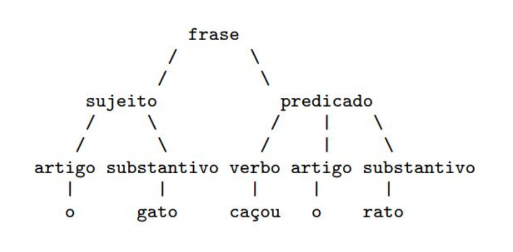
\includegraphics{figuras/figura-1_arvore.png}
    \Fonte{Extraído de \cite{do2019processamento}.} 
    \label{fig:sintaxe}
\end{figure}

A semântica associa significado a uma estrutura sintática, em termos dos significados das palavras que a compõem (e.g. à estrutura da Figura \ref{fig:sintaxe}, podemos associar o significado “um animal 
perseguiu/capturou outro animal”) \cite{de2019unidades}. Finalmente, a pragmática verifica se o significado 
associado à uma estrutura sintática é realmente o significado mais apropriado no contexto considerado (e.g. 
no contexto predador-presa, “perseguiu/capturou” → “comeu”) \cite{moro2018reconhecimento}.

Mesmo com o avanço no relacionamento homem-máquina, a comunicação via linguagem natural continua sendo um 
desafio: como criar programas capazes de interpretar mensagens codificadas em linguagem natural e decifrá-
las para a linguagem de máquina? \cite{silva2021detecccao} Ao longo dos anos, muitas pesquisas e 
desenvolvimentos ocorreram nos mais diversos ramos do processamento de linguagem natural, com ênfase na 
sumarização automática, que a maioria considera ser o ponto de partida para o estudo da linguagem natural 
por meio de computadores \cite{rodriguez2020processamento}.

Para modelar uma linguagem e permitir que as máquinas a compreendam, é necessário um processo de pré-processamento abstrato e estruturado para deixar apenas informações relevantes. Esse pré-processamento reduz o tamanho do vocabulário e torna os dados menos esparsos, um recurso conveniente do processamento computacional \cite{de2020mike}.

A seguir serão descritas as técnicas de processamento da linguagem natural, que são a Normalização (Seção \ref{sec:normalizacao}), Remoção de \textit{Stopwords} (Seção \ref{sec:remocao-stopwords}), Remoção de Numerais (Seção \ref{sec:remocao-numerais}), \textit{Stemização} e Lematização (Seção \ref{sec:stemizacao-lematizacao}), Compreensão da Linguagem Natural (seção \ref{sec:compreensao-linguagem-natural}), e na Seção \ref{sec:terminologia-utilizada} serão descritas as terminologias utilizadas, que são \textit{Tokenização} (Seção \ref{sec:tokenizacao}), Mineração de Textos (Seção \ref{sec:mineracao-textos}) e a Sumarização Automática (Seção \ref{sec:sumarizacao-automatica}).

\subsection{Normalização}
\label{sec:normalizacao}
A normalização abrange tratativas como a \textit{tokenização} \cite{de2022processamento}, transformação de letras 
maiúsculas para minúsculas, remoção de caracteres especiais, remoção de \textit{tags} HTML/Javascript/CSS, 
dentre outras \cite{motta2018estudo}. O processo de \textit{tokenização} visa dividir palavras ou frases em unidades. A \textit{tokenização} lexical \textit{tokeniza} cada palavra como um \textit{token} no texto, reconhecendo-a mesmo que seja tocada por sinais de pontuação \cite{cidrimtecnologias}. 
Um exemplo de texto \textit{tokenizado} lexicalmente seria:
\begin{itemize}
	\item Esta é uma sentença.
	\item[] ['Esta', 'é', 'uma', 'sentença', '.']
\end{itemize} 

A \textit{tokenização} sentencial identifica e marca sentenças. Um exemplo seria:
\begin{itemize}
	\item Esta é a primeira sentença. Esta é a segunda. Esta é a terceira!
	\item[] ['Esta é a primeira sentença.', 'Esta é a segunda.', 'Esta é a terceira!']
\end{itemize}

A normalização é importante por começar a estruturar o texto, já que os processamentos seguintes atuam a partir de unidades sentenciais e lexicais \cite{pinho2021analise}.

\subsection{Remoção de \textit{Stopwords}}
\label{sec:remocao-stopwords}
Uma das tarefas muito utilizadas no pré-processamento de textos é a remoção de \textit{stopwords}. Esse 
método consiste em remover palavras muito frequentes, tais como “a”, “de”, “o”, “da”, “que”, “e”, “do” 
entre outras, pois na maioria das vezes não são informações relevantes para a construção do modelo 
\cite{dos2021analise}. 
Esse processo, só pode ser aplicado quando realmente as palavras não forem importantes para a compreensão do 
sentido do texto.

\subsection{Remoção de Numerais}
\label{sec:remocao-numerais}
Outra remoção necessária é a dos numerais presentes no texto. Os numerais não agregam informação relevante 
por não trazerem carga semântica \cite{jurafskymartin2020}. O PLN remove também os símbolos que os 
acompanham, como “R\$”, “\$”, “US\$”, “km”, “milhões”, “bilhões”, dentre outros.

\subsection{Stemização e Lematização}
\label{sec:stemizacao-lematizacao}
O processo de \textit{stemização} (do inglês, \textit{stemming}) consiste em reduzir uma palavra ao seu 
radical \cite{gobbo2019abordagem}. A palavra “meninas” se reduziria a “menin”, assim como “meninos” e 
“menininhos”. As palavras “gato”, “gata”, “gatos” e “gatas” reduzem-se para “gat”. A lematização reduz a 
palavra ao seu lema, que é a forma no masculino e singular. No caso de verbos, o lema é o infinitivo 
\cite{campos2021uso}.

Por exemplo, as palavras “gato”, “gata”, “gatos” e “gatas” são todas formas do mesmo lema: “gato”. 
Igualmente, as palavras “tiver”, “tenho”, “tinha”, “tem” são formas do mesmo lema “ter”. A vantagem de 
aplicar a \textit{stemização} ou lematização é clara: redução de vocabulário e abstração de significado
\cite{santos2022processamento}.

\subsection{Compreensão da Linguagem Natural}
\label{sec:compreensao-linguagem-natural}
Essa parte do processamento de linguagem natural é responsável por transformar sentenças de um texto em 
estruturas lógicas, ou seja, é compreender uma frase que carrega um valor que pode ser verdadeiro ou falso 
\cite{frutuoso2018processamento}.

A compreensão da linguagem natural tem como objetivo facilitar a manipulação de texto por computadores, além 
de identificar instruções recebidas por humanos e até por outras máquinas. É o processo de construção de uma 
base semântica formal da linguagem. O significado atribuído a sentenças pode ser interpretado pelo 
computador, da mesma forma que os humanos o fazem \cite{d2022inteligencia}.

\section{Terminologia Utilizada}
\label{sec:terminologia-utilizada}
Esta seção, apresenta as principais terminologias utilizadas no decorrer dessa pesquisa.

\subsection{Tokenização}
\label{sec:tokenizacao}
Uma das principais etapas da operação de normalização é a \textit{tokenização}, que é realizada com o objetivo de quebrar um documento de texto nas menores unidades, mas que representem a mesma semântica original do texto. É usado durante o processamento de linguagem natural para segmentação de palavras, localizando caracteres para quebrar sequências de caracteres no texto Limites por palavra, ou seja, palavras separadas ou frases em unidades \cite{rodriguez2020processamento}.

A \textit{tokenização} também foi exemplificada na Seção \ref{sec:normalizacao}.

\subsection{Mineração de Textos}
\label{sec:mineracao-textos}
A mineração de textos é um conjunto de métodos utilizado para navegar, organizar, encontrar e descobrir informações em bases textuais \cite{deuso}.

A tecnologia de mineração de textos deriva das técnicas de recuperação de informações e da descoberta de informações estruturadas, por meio do uso de bancos de dados e de procedimentos estatísticos \cite{lima2022big}. É uma subárea da extração de informações, porém é utilizada somente para análise em textos.

Por mais que possa parecer similar, a mineração de textos é diferente de mecanismos de busca, uma vez que 
na busca o usuário já sabe o que quer encontrar; enquanto na mineração de textos, o usuário descobrirá conhecimento e padrões até então, por ele desconhecidos \cite{souza2021modelo}. Em suma, na busca o usuário pesquisa determinada informação e na mineração é realizada a coleta de novos conhecimentos “escondidos” nos textos.

Mineração de textos \cite{ferreira2021mineraccao} é o processo de extrair conhecimento não conhecido previamente a partir de fontes textuais, tais como correio, imprensa, transações, \textit{websites}, \textit{newsgroups}, fóruns, listas de correspondência, redes sociais, dentre outros.

\subsection{Sumarização Automática}
\label{sec:sumarizacao-automatica}
A sumarização automática é o processo de selecionar as informações mais importantes de um conjunto de
fontes, seja um único texto ou um corpus, para produzir uma versão resumida \cite{martins2001introduccao}.

Os textos podem ser de qualquer tipo: notícias, artigos científicos, postagens em blogs, resenhas de filmes, atas de reuniões e muito mais. Eles também podem ser escritos em qualquer idioma sem a necessidade de uma escrita formal ou casta. Obviamente, os métodos de resumo, incluindo algum pré-processamento, podem variar de idioma para idioma, com a grande maioria existente para o inglês \cite{cabral2014platform}.

Computacionalmente explicando, existem duas formas de se abordar o problema da sumarização, a superficial e
a profunda \cite{salvino2019analise}. Neste trabalho será abordada a primeira, que utiliza métodos 
estatísticos e/ou empíricos para obter o sumário. Essa técnica é a mais simples de ser implementada e é 
utilizada por grande parte dos pesquisadores, porém, pode produzir sumários com problemas de coesão e 
principalmente de coerência, o que pode deixar o resumo sem um sentido lógico da ordem das frases, 
apresentando deficiências no sentido das frases \cite{antunes2018abordagem}. Por outro lado, a sumarização profunda realiza uma análise semântica frase a frase no texto, analisando a forma que as frases são 
construídas e o relacionamento de uma frase a outra \cite{pinho2021analise}.

\section{Trabalhos Relacionados}
\label{sec:relatedWork}
Esta seção, visa apresentar alguns trabalhos relacionados ao Processamento de Linguagem Natural.
%
Em \citeonline{singh2018natural}, são apresentadas as sub-tarefas da tecnologia de extração de informações, 
além de destacar pesquisas de ponta em várias tarefas onde a extração de informação é utilizada. Além disso, 
o artigo destaca os desafios atuais de lidar com o Processamento de Linguagem Natural, em razão da explosão 
de informações na forma de notícias, artigos, redes sociais, mídia, de uma forma que todo o texto 
interpretado pela máquina consiga ser identificado, extraído e repassado para o usuário de uma forma 
entendível.

\citeonline{rodriguez2020processamento} apresentam uma forma alternativa de integração do meio jurídico com a 
tecnologia, expondo meios de como o Processamento de Linguagem Natural poderia ajudar a automatizar o 
reconhecimento de Entidades Nomeadas (Agentes Públicos) em uma base de portaria. Eles utilizam o NLTK 
(\textit{Natural Language Toolkit}), que junto da linguagem de programação \textit{Python}, trabalham com 
dados de linguagem humana para aplicação do PNL. O NLTK é útil para separar as sentenças em um paragrafo, 
separar as palavras dentro de cada sentença, reconhecer padrões no texto e criar modelos de classificação que 
permitam identificar nomes próprios dentro de um conjunto de dados.

\citeonline{vieira2019analise} apresentam uma análise descritiva acerca do conteúdo das notícias publicadas 
no Portal da Saúde, através da utilização da técnica de mineração de textos, onde tentam gerar insumos e 
informações para discussões sobre o impacto da \textit{fake news} na área da saúde. A ideia vem da análise de 
uma iniciativa lançada pelo Ministério da Saúde sobre o enfrentamento de notícias falsas que tem se espalhado 
nas mais diversas áreas, como política, finanças e a própria saúde, que se chama "Saúde sem 
\textit{fake news}".

\citeonline{tabosa2020avaliaccao} apresenta uma pesquisa iniciada no ano de 2014 sobre o desenvolvimento de 
um \textit{software} que fosse capaz de criar resumos automáticos de textos baseados em técnicas de PLN, 
baseando-se na frequência de palavras. Os primeiros testes dessa ferramenta geraram resultados que indicavam 
uma significativa redução da dimensionalidade dos textos, preservando seu valor semântico. O artigo apresenta 
os resultados dessa pesquisa mostrando que existiu uma equivalência qualitativa entre os resumos produzidos 
pela ferramenta e por humanos, mas que deixa a desejar quando se trata do tamanho do resumo gerado, visto que 
o resultado da sumarização feita pela ferramenta denota textos muito longos.

O algoritmo de Marques apresentado neste trabalho foi comparado com outros algoritmos de sumarização automática de texto presentes na literatura. Dentre os trabalhos relacionados, destacam-se os algoritmos GistSumm, Luhn, PLI, Regressão Bayesiana e ChatGPT. A Tabela  \ref{tab:comparacao_marques_trabalhos_relacionados} apresenta as principais diferenças entre o algoritmo de Marques e os algoritmos relacionados.

O algoritmo de Marques se destaca em relação aos algoritmos relacionados por utilizar um modelo de redes neurais treinado especificamente para a tarefa de sumarização automática de textos.

\begin{table}[ht]
\centering
\caption{Comparação entre o algoritmo de Marques e algoritmos relacionados}
\label{tab:comparacao_marques_trabalhos_relacionados}
    \begin{tabular}{|l|p{6cm}|p{6cm}|}
    \hline
        \textbf{Algoritmo} & \textbf{Características} & \textbf{Diferenciais em relação ao algoritmo de Marques} \\ \hline
        GistSumm & Baseado em técnicas de extração & Menor desempenho em precisão, coerência e coesão \\ \hline
        Luhn & Utiliza frequência de palavras e posição no texto & Inferior em termos de precisão e coerência \\ \hline
        PLI & Baseado em programação linear inteira & Desempenho inferior nas métricas de qualidade \\ \hline
        Regressão Bayesiana & Abordagem baseada em aprendizado de máquina & Tempo de processamento mais lento \\ \hline
        ChatGPT & Geração de resumos por modelo pré-treinado de linguagem & Tempo de processamento mais lento e desempenho inferior nas métricas de qualidade \\ \hline
        Marques & Redes neurais treinadas especificamente para sumarização automática de textos & Melhor desempenho em precisão, coerência, coesão e tempo de processamento \\ \hline
    \end{tabular}
\end{table}
	\chapter{Materiais e Métodos}
\label{chap:materiais-e-metodos}

Neste capítulo, são apresentadas as principais tecnologias e ferramentas empregadas ao longo deste 
trabalho, bem como uma descrição detalhada dos algoritmos estudados. A Seção \ref{sec:python} aborda a 
linguagem de programação empregada no desenvolvimento do algoritmo proposto por Marques. A Seção 
\ref{chap:algoritmos-trabalhados} discute os algoritmos que serão comparados ao método desenvolvido pelo 
autor. Por fim, a Seção \ref{cap:projeto_experimento} descreve a metodologia experimental adotada e explica 
como o experimento foi conduzido.

\section{Python}
\label{sec:python}
Python é uma linguagem de programação interpretada de alto nível e que suporta múltiplos paradigmas de 
programação: imperativo, orientado a objetos e funcional. É uma linguagem com tipagem dinâmica e 
gerenciamento automático de memória \cite{pereira2020sistema}.

A linguagem \textit{Python} foi escolhida pela facilidade de criar e manusear uma Inteligência Artificial (IA), que deixa o desenvolvimento mais fluído e de forma mais orgânica \cite{deolhar}.

\section{Algoritmos Trabalhados}
\label{chap:algoritmos-trabalhados}

Neste trabalho, foram analisados e avaliados os algoritmos de Luhn \cite{luhn1957stoical}, \textit{GistSumm} \cite{gistsumm}, o algoritmo de Programação Linear Inteira \cite{oliveira2018sumarizaccao}, um algoritmo de regressão Bayesiana \cite{sodre2019avaliando}, o \textit{ChatGPT} \cite{rudolph2023chatgpt} e um algoritmo criado pelo pesquisador dessa monografia, todos sumarizadores baseados na extração de palavras-chave do texto. 

O algoritmo de Luhn é um dos trabalhos mais importantes na área de PLN, em Sumarização de Documentos \cite{luhn1957stoical}, é um algoritmo clássico que serviu como base para muitos algoritmos, seu método de extração é baseado na extração de palavras-chave.

Os algoritmos citados anteriormente são embasados no algoritmo de Luhn, mas desenvolvidos a partir de abordagens distintas, como técnicas de regressão, inferências Bayesianas, além de mostrarem que utilizando a sentença principal do texto é mais eficiente quando se trata de gerar resumos com as ideias principais de um texto \cite{salvino2019analise}.

Os algoritmos estudados são mais utilizados para sumarizar textos que não são monografias, artigos, pesquisas cientificas e outros dentro dessa área.

Além de analisar os principais desafios da área de sumarização automática de textos, o objetivo deste trabalho é a criação de um algoritmo que se destine especificamente à produção de resumos de textos acadêmicos, como monografias, artigos e pesquisas. Dessa forma, busca-se contribuir com a comunidade científica, fornecendo uma ferramenta que facilite a criação literária e pesquisa, ao mesmo tempo em que se avança no conhecimento sobre a área de sumarização automática de textos.

\section{Projeto do Experimento}
\label{cap:projeto_experimento}

Esta seção, descreve o planejamento e execução do experimento de comparação dos algoritmos, com o objetivo de determinar qual deles melhor atende às expectativas do usuário.

\subsection{Instrumentação}
\label{chap:instrumentacao}

A instrumentação dos experimentos é dividida em hardware e software. Será utilizado um computador equipado com um processador Intel Core i5-10500H (10ª geração) \textit{Quad Core} para executar um conjunto de códigos-fonte em \textit{Python} 3.10, que implementam os algoritmos a serem avaliados.

\subsection{Etapas do Experimento}
\label{chap:experimento}

O experimento é composto por três etapas, conforme ilustrado na Figura \ref{fig:projeto-experimento}:

\begin{figure}[!h]
\centering
    \caption{Etapas do Experimento}
    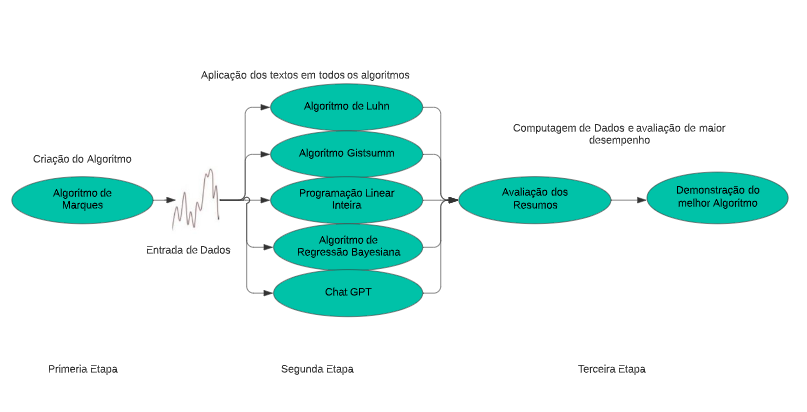
\includegraphics[width=\textwidth]{figuras/design-experimento.png}
    \label{fig:projeto-experimento}
    \Fonte{Autoria própria.}
\end{figure}

A avaliação de desempenho dos algoritmos foi realizada com base em métricas como taxa de coerência, taxa de coesão, precisão e tempo de processamento. Essas métricas são amplamente utilizadas na literatura para avaliar a qualidade dos resumos gerados por algoritmos de sumarização automática de texto \cite{pandian2021performance}. A seguir, serão apresentadas as definições e explicações detalhadas de cada métrica utilizada.
\begin{itemize}
    \item Coerência: A taxa de coerência avalia a lógica e a clareza da     estrutura do resumo gerado. Um resumo coerente deve apresentar as informações de maneira lógica, com uma sequência que faça sentido e     seja fácil de seguir pelo leitor. A coerência pode variar de 0 a 1, sendo que valores mais próximos de 1 indicam maior coerência no resumo gerado.

    \item Coesão: A taxa de coesão mede o grau de conexão entre as ideias presentes no resumo gerado. Um resumo coeso deve apresentar ideias relacionadas de maneira integrada e harmoniosa, sem lacunas ou informações desconexas. A coesão também pode variar de 0 a 1, sendo que valores mais próximos de 1 indicam maior coesão no resumo gerado.

    \item Precisão: A precisão avalia a capacidade do algoritmo em selecionar as informações mais relevantes do texto original para 
    compor o resumo. Um resumo preciso deve conter as informações 
    essenciais e mais importantes do texto original, sem incluir 
    informações desnecessárias ou irrelevantes. A precisão pode variar 
    de 0 a 1, sendo que valores mais próximos de 1 indicam maior 
    precisão na seleção de informações relevantes para o resumo.

    \item Tempo de processamento: O tempo de processamento é uma medida 
    do tempo necessário para que o algoritmo processe o texto original e gere o resumo correspondente. Essa métrica é importante para avaliar a eficiência dos algoritmos em termos de rapidez e capacidade de processar grandes volumes de dados. O tempo de processamento é geralmente expresso em segundos, sendo que menores valores indicam um algoritmo mais rápido e eficiente.
\end{itemize}

A análise dessas métricas, fundamentada em estudos prévios e na literatura científica sobre sumarização automática, possibilita uma compreensão aprofundada do desempenho dos algoritmos de sumarização automática. Essa análise fornece informações valiosas para a seleção do algoritmo mais adequado, levando em consideração as necessidades específicas dos usuários.

A Etapa 1 envolve a criação do algoritmo de Marques. Na Etapa 2, o objetivo é realizar a sumarização automática de um artigo sobre a pandemia da COVID-19 e as mudanças no estilo de vida dos brasileiros adultos (\cite{MALTA2020}). O texto que servirá de base para a geração dos resumos está disponível no Anexo \ref{chap:texto_covid} e será processado através de seis algoritmos distintos. Por fim, na Etapa 3, os resumos serão avaliados por um grupo de avaliadores, que julgarão a qualidade dos resumos gerados por cada algoritmo, a fim de determinar o desempenho de cada um deles.

O cenário considerado para os experimentos envolve a simulação de resumos em uma máquina virtual com capacidade de processamento de um Intel Core i5 10500H (10ª geração) – 12 MB de cache, 6 núcleos e 12 \textit{threads} – com frequência de 2.50 GHz até 4.50 GHz e 16 GB de memória RAM. A análise das sumarizações obtidas será realizada dentro de um contexto educacional.

\subsubsection{Etapa 1: Criação do Algoritmo de Marques}
\label{chap:primeira-etapa}

A primeira etapa consiste na criação do algoritmo de Marques, que começa criando uma matriz do texto, dividindo-o em sentenças e, em seguida, em palavras. Então, identifica palavras com função sintática, mas sem relevância semântica, como "ou", "e", "para", e as remove da matriz. Isso é feito porque essas palavras são frequentes e acabariam recebendo importância indevida, dificultando a análise textual. Pontuações também são removidas, pois o algoritmo as trata como palavras, o que atrapalha a sumarização.

Após a limpeza do texto, o algoritmo cria uma distribuição de frequência para a matriz de palavras, identificando as mais importantes. Com base nessa distribuição, o algoritmo seleciona as palavras mais comuns, de acordo com um valor pré-determinado, para posteriormente classificá-las como relevantes ou não no resumo final.

\subsubsection{Etapa 2: Sumarização Automática}
\label{chap:segunda-etapa}

A segunda etapa, consiste em realizar a sumarização automática usando os algoritmos de Luhn, \textit{Gistsumm}, PLI \cite{oliveira2018sumarizaccao}, regressão Bayesiana, \textit{ChatGPT} e o algoritmo de Marques.

Foram realizados testes nas configurações dos parâmetros comuns modificáveis nos algoritmos, isto é, na quantidade de sentenças importantes, a fim de equipará-los para a etapa seguinte. Dessa forma, neste experimento foi utilizado o parâmetro de \textbf{cinco (5) sentenças importantes}.

Segundo \citeonline{rino2003sumarizaccao}, para gerar um resumo eficiente, deve-se extrair entre 20 a 50\% do texto e atingir uma taxa de compressão de 80\%. Neste trabalho, seguimos essa orientação ao avaliar os algoritmos de sumarização automática.

Considerando os parâmetros mencionados, o texto utilizado no resumo seguiu uma taxa de compressão de aproximadamente 40\% para cada algoritmo. O algoritmo de Marques, por exemplo, selecionou as cinco sentenças mais importantes do texto original, que representam uma porcentagem significativa das informações relevantes. Essas cinco sentenças foram determinadas com base na frequência das palavras e na relevância das sentenças no contexto do texto.

As cinco sentenças importantes servem como um critério para avaliar a qualidade dos resumos gerados pelos algoritmos de sumarização automática. A escolha dessas sentenças permite obter um resumo conciso e informativo, mantendo a essência do texto original e assegurando que o leitor compreenda os principais pontos abordados. Esse critério contribui para a eficiência dos resumos gerados e auxilia na comparação dos algoritmos em relação à sua capacidade de extrair informações relevantes e concisas do texto original \cite{oliveira2022composiccao}.

\subsubsection{Etapa 3: Avaliação dos Resumos}
\label{chap:terceira-etapa}

Para avaliar a qualidade e coesão dos resumos gerados na segunda etapa, foram coletadas 49 respostas 
de indivíduos com diferentes graus de instrução acadêmica que responderam a questionários aleatórios. Essas pessoas avaliaram os resumos resultantes da inserção do artigo de \citeonline{MALTA2020} distribuídos entre 6 resumos e 5 questionários, comparando cada algoritmo mencionado na segunda etapa com o algoritmo de Marques.

Os avaliadores julgaram qual texto apresentava maior coesão e coerência, sem saber quais algoritmos foram utilizados. Em todos os casos, o texto 1 representa o resumo proveniente do algoritmo de Marques, enquanto o texto 2 em cada questionário representa os algoritmos comparados: Luhn, \textit{Gistsumm}, PLI \cite{oliveira2018sumarizaccao}, regressão Bayesiana e \textit{ChatGPT}.

Os questionários foram enviados por meio de formulários no \textit{Google Docs}, conforme modelo apresentado no Apêndice \ref{ap:Forms}.

\subsection{Amostragem e Seleção dos Participantes}
\label{subsec:amostragem}

A escolha dos participantes para a avaliação dos algoritmos de sumarização automática neste trabalho foi feita através de uma amostragem por conveniência. A amostragem por conveniência é uma técnica não probabilística que seleciona os participantes com base na disponibilidade e na facilidade de acesso \cite{neuman2006workbook}.

Os questionários foram preenchidos pelos participantes após a divulgação dos formulários pelas redes sociais do autor e do orientador. Esse método de seleção permitiu alcançar um grupo diversificado de participantes, embora não seja uma amostra totalmente representativa da população em geral.

É importante mencionar que a amostragem por conveniência pode ter sido influenciada pelo efeito \textit{snowball} \cite{goodman1961snowball}. O efeito \textit{snowball} ocorre quando os participantes iniciais compartilham o questionário com seus contatos, que por sua vez compartilham com seus próprios contatos, aumentando o alcance da pesquisa. Esse efeito pode introduzir viés na amostra, uma vez que as pessoas que participam da pesquisa tendem a ter características semelhantes ou estarem 
relacionadas de alguma forma.

Apesar dessas limitações, a amostragem por conveniência e o possível efeito \textit{snowball} permitiram obter um número suficiente de respostas para a avaliação dos algoritmos de sumarização automática, fornecendo informações valiosas sobre o desempenho dos algoritmos em relação às métricas estabelecidas.

Após a coleta das respostas, os resultados foram processados e analisados com base em métricas específicas de qualidade de sumarização, como precisão, coerência e coesão, além do tempo de processamento. Essa análise permitiu determinar qual algoritmo apresentou melhor desempenho na geração de resumos coerentes e coesos. Os algoritmos utilizados na comparação e seus respectivos métodos de sumarização serão detalhados no capítulo \ref{cap:algoritmos}.
	\chapter{Algoritmos de Sumarização de Texto}
\label{cap:algoritmos}

Este capítulo, explica os algoritmos utilizados nessa monografia que, por meio de uma pesquisa, comparará cada um destes algoritmos consolidados com o proposto pelo autor do presente trabalho.

\section{Algoritmo de Luhn}
\label{chap:Algluhn}
O algoritmo de Luhn analisa as frases mais importantes de um documento, que são aquelas que mais aparecem no 
texto. Neste contexto, não são consideradas as \textit{stopwords}, que são palavras como artigos, preposições, 
conjunções, entre outras que aparecem com frequência em um texto, porém são insignificantes em relação ao 
significado semântico do documento \cite{da2022mineraccao}. Em suma, as \textit{stopwords} são utilizadas apenas 
para dar um sentido gramatical correto na formação das frases. Como o algoritmo faz a sumarização baseada na 
frequência que as palavras ocorrem, elas são desconsideradas para não confundir o sumarizador.

\begin{figure}
    \centering
    \caption{Modelo de Funcionamento do Algoritmo de Luhn}
    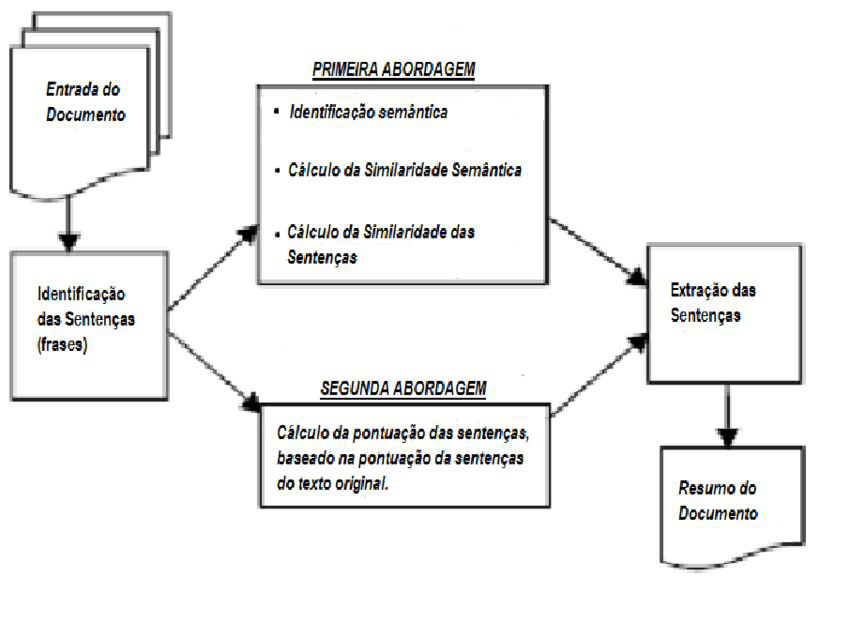
\includegraphics[width=.8\textwidth]{figuras/luhn-funcionamento.png}
    \Fonte{Extraído de \cite{russell2011mineraccao}.} 
    \label{fig:luhn-figure}
\end{figure}

O algoritmo não procura compreender os dados em um nível semântico, e simplesmente computa resumos com 
agrupamento de palavras que ocorrem com frequência no texto. A Figura \ref{fig:luhn-figure} apresenta os 
passos desde quando o algoritmo de Luhn recebe um texto como parâmetro até a geração final do resumo. A 
primeira tarefa é identificar as frases, calculando a similaridade entre todas as frases do texto. Na 
segunda abordagem, outra tarefa é fazer o cálculo da pontuação, levando em conta que o resumo nunca pode ter 
mais pontos e vírgulas que o texto original. Terminadas a primeira e segunda abordagens mostradas na Figura 
\ref{fig:luhn-figure}, o algoritmo finalmente extrai as sentenças escolhidas, as agrupa e mostra como resultado o resumo. O resumo gerado pelo algoritmo de Luhn está no anexo \ref{chap:luhn_resumo}

O algoritmo de Regressão Bayesiana é uma releitura do Algoritmo de Luhn, funcionando conforme descrito anteriormente. O resumo gerado pelo algoritmo de Regressão Bayesiana está no anexo \ref{chap:bayesiana_resumo}.


\section{Algoritmo Gistsumm}
\label{chap:Alggistsumm}
O \textit{GistSumm} (\textit{GistSumarizer}) é um sumarizador extrativo que usa técnicas estatísticas para determinar a ideia central dos textos por ele sumarizados. Baseia-se na simulação da sumarização humana, primeiro identificando a ideia principal do texto e, então, acrescenta informações adicionais ou complementares \cite{brewka1996artificial}. Essas informações adicionais podem ser a segunda ou terceira frase mais importante do texto, seguindo em ordem crescente de acordo com a quantidade de frases que se deseja extrair do texto.

Dessa forma, o sumarizador primeiro procura a sentença que melhor expressa a ideia principal do texto e baseado nela são escolhidas as demais sentenças, que vão compor o extrato textual. Mesmo quando a sentença escolhida não for a sentença principal e há uma aproximação significativa da mesma, o extrato já pode ser gerado \cite{torres2014automatic}. 

O \textit{GistSumm} compreende três processos principais, e mais alguns secundários, os quais são descritos a seguir: segmentação textual, ranqueamento de sentenças e seleção de sentenças.

A segmentação textual delimita as sentenças do texto-fonte e procura pelos sinais de pontuação. O ranqueamento é uma ordenação a partir de pesos obtidos na aplicação de métodos estatísticos, sendo feita a análise léxica, extração das \textit{stopwords} e aplicação do método de ranqueamento. Por fim, a seleção de sentença escolhe as sentenças mais relevantes, por meio de seus métodos extrativos, para, deste modo, gerar o sumário do documento analisado \cite{muller2015comparativo}. Neste momento, o texto é transformado de acordo com a taxa de compressão definida. A taxa de compressão é a porcentagem do texto original que o algoritmo pode extrair para o resumo.
O resumo gerado pelo algoritmo \textit{Gistsumm} está no anexo \ref{chap:gistsumm_resumo}.


\section{Algoritmo de Programação Linear Inteira (PLI)}
\label{sec:algoritmo-oliveira}

O Algoritmo de programação Linear Inteira tem como objetivo a sumarização automática de textos baseada em conceitos, utilizando programação linear inteira e regressão. Essa abordagem busca extrair as informações mais importantes de um texto e gerar um resumo coerente e relevante. O PLI segue as etapas:

\subsection{Pré-processamento}
Nesta etapa, o texto é pré-processado para eliminar ruídos e facilitar a extração de informações. O pré-processamento inclui a remoção de pontuação, números, caracteres especiais e \textit{stopwords}, além da normalização do texto, como a conversão de todas as letras para minúsculas e a redução das palavras ao seu radical (\textit{stemming}).

\subsection{Extração de Conceitos}
Com base no texto pré-processado, os conceitos são extraídos. Um conceito é uma palavra ou expressão que representa uma ideia importante no texto. A frequência de cada conceito no texto é calculada, e os conceitos são ordenados de acordo com sua importância, considerando suas frequências e pesos semânticos.

\subsection{Seleção de Sentenças}
Nesta etapa, as sentenças que contêm os conceitos mais importantes são selecionadas para compor o resumo. O algoritmo utiliza programação linear inteira para determinar a melhor combinação de sentenças que maximiza a cobertura dos conceitos importantes, mantendo a coerência e a concisão do resumo. A programação linear inteira é uma técnica matemática que permite a resolução de problemas de otimização com variáveis inteiras.

\subsection{Regressão}
A regressão é aplicada para ajustar os pesos dos conceitos e das sentenças, de forma a melhorar a qualidade do resumo gerado. O algoritmo utiliza um conjunto de treinamento com textos e resumos previamente avaliados por humanos para aprender a importância relativa dos conceitos e sentenças no processo de sumarização. A regressão permite que o algoritmo ajuste seus parâmetros de acordo com os padrões observados nos dados de treinamento, melhorando a precisão e a relevância dos resumos gerados.

\subsection{Geração do Resumo}
Com base na seleção de sentenças e nos pesos ajustados dos conceitos, o resumo final é gerado. As sentenças selecionadas são reorganizadas de acordo com a ordem em que aparecem no texto original, garantindo a coerência e a fluidez do resumo.

O PLI apresenta uma abordagem interessante para a sumarização automática de textos, combinando técnicas de programação linear inteira e regressão para extrair e ponderar conceitos importantes e selecionar as sentenças mais relevantes para compor o resumo. Essa abordagem busca gerar resumos mais precisos, coerentes e informativos, levando em consideração a importância dos conceitos e a estrutura do texto original.
O resumo gerado está no anexo \ref{chap:pli_resumo}.


\section{\textit{ChatGPT}}
\label{chap:chatgpt}

O \textit{ChatGPT} é um algoritmo baseado em inteligência artificial, criado pela \textit{OpenAI} \cite{lund2023chatting}. Seu nome vem é uma sigla de \textit{Generative Pre-Trained Transformer}, que significa, em tradução livre, Transformador pré-treinado generativo \cite{transformer2022rapamycin}. Esse algoritmo tem seu desenvolvimento traçado a partir de redes neurais e \textit{Machine Learning}, e tem foco semelhante a \textit{chatbots}, com conversação online. A ideia a partir do que ele foi criado, é para aprimorar a experiência e recursos oferecidos por alguns assistentes virtuais, como Alexa, Google Assistente, dentre outros. Grande parte de ter se tornado famoso e ter tanto sucesso se dá pela forma simples de conversação e obtenção de respostas \cite{aydin2023ChatGPT}.

A sua arquitetura se baseia em uma rede neural chamada \textit{Transformer}, que é projetada especialmente para lidar com textos. Seu modelo de várias camadas permite que a plataforma consiga identificar palavras-chave, nos mais diferentes contextos inseridos \cite{natarajan2020wide}. Esse algoritmo se alimenta de informações que colhe da Internet. Nesse caso, tudo que existe hoje disponível na rede pode ser usado como base para essa ferramenta \cite{rao2023assessing}. Seguindo alguns padrões e no cruzamento de informações, o \textit{ChatGPT} transforma as \textit{querys}, perguntas feitas pelo usuário, em respostas. Seu diferencial se dá na criatividade que está presente nessas respostas, já que, diferente dos métodos tradicionais de busca, ele traz a resposta contextualizada e em um texto elaborado que busca o maior entendimento do leitor, além da possibilidade de elaborar musicas, poesias, códigos de programação, receitas, dentre outras \cite{rudolph2023chatgpt}.
O resumo gerado pelo \textit{ChatGPT} está no anexo \ref{chap:chatgpt_resumo}.


\section{Algoritmo de Marques}
\label{chap:marques}
O algoritmo proposto pelo autor tem embasamento no algoritmo \textit{GistSumm} (\textit{GistSumarizer}), que é embasado no algoritmo de Luhn, e seu método de extração de palavras-chave baseado na sentença principal do texto é muito eficiente quando trata-se de gerar resumos com as ideias principais de um texto \cite{castro2022extraccao}. De acordo com \citeonline{rino2003sumarizaccao}, o \textit{GistSumm} atualmente encontra-se como o estado da arte de sumarização automática de documentos, com uma função para sumarização multi-documentos.

Segundo o trabalho de \citeonline{de2011blmsumm}, a eficiência de um algoritmo de sumarização está ligada ao desempenho de seu método de extração de palavras-chave. Para verificar essa hipótese, serão utilizadas tabelas com os resultados, essas tabelas mostram todos os dados tanto em forma numérica e percentual, onde podemos perceber a eficiência e demais características dos algoritmos, tais como taxa de erros e acertos. Avaliações de forma semelhante a essas foram feitas nos trabalhos de Luhn e \citeonline{rino2003sumarizaccao}, sendo que somente o trabalho de \citeonline{rino2003sumarizaccao} aplica-se ao português do Brasil.

O algoritmo de Marques é um sumarizador extrativo que usa técnicas estatísticas para determinar a ideia central dos textos por ele sumarizados, que implementa bibliotecas da linguagem \textit{Python} 3.10. Baseia-se na simulação da sumarização humana, primeiro identificando a ideia principal do texto e, então, acrescenta informações adicionais ou complementares. Essas informações adicionais podem ser a segunda ou terceira frase mais importante do texto, seguindo em ordem crescente de acordo com a quantidade de frases que se deseja extrair do texto.

Dessa forma, o sumarizador primeiro procura a sentença que melhor expressa a ideia principal do texto, e baseado nela são escolhidas as demais sentenças que vão compor o extrato textual. O \textit{GistSumm} trabalha da mesma forma: primeiro o GistSumm realiza a identificação da sentença principal com o uso de métodos estatísticos simples, e, por segundo, conhecendo-se as sentenças principais é possível produzir extratos coerentes. Mesmo quando a sentença escolhida não for a sentença principal e há uma aproximação significativa da mesma, o extrato já pode ser gerado.
O código do algoritmo de Marques está no apêndice \ref{chap:marques_algoritmo}.
O resumo gerado pelo algoritmo de Marques está no apêndice \ref{chap:marques_resumo}.
    \chapter{Resultados e Discussões}
\label{chap:resultados}
Este capítulo, apresenta os resultados obtidos através da análise comparativa dos seis algoritmos de sumarização automática de texto descritos no Capítulo \ref{cap:algoritmos}. A metodologia utilizada consistiu na aplicação dos algoritmos em um texto sobre a COVID-19 e seus impactos na pandemia \cite{MALTA2020}, e na avaliação dos resultados com base em métricas de qualidade de sumarização.

\section{Comparativo dos Algoritmos}
\label{chap:comparativo}
Esta seção, apresenta os resultados obtidos para cada um dos algoritmos, sendo comparados com o algoritmo de Marques. Foram obtidas 49 respostas ao total. Vale salientar que os respondentes são todos distintos (49).

A fim de organização, nos gráficos, o texto \textbf{um} sempre será o algoritmo de Marques, e o texto \textbf{dois} o algoritmo daquela seção.

\subsection{Algoritmo de Luhn}
\label{chap:luhn}

\begin{figure}[h]
    \centering
    \caption{Respostas ao Questionário sobre Marques x Luhn}
    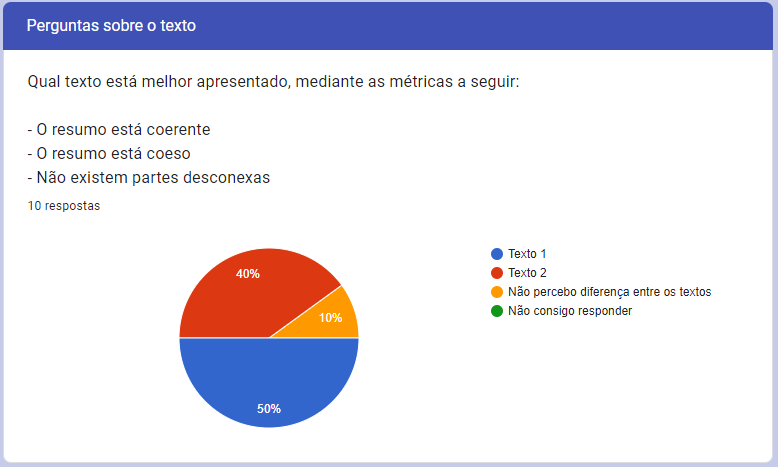
\includegraphics[width=\textwidth]{figuras/graficos/luhn.png}
    \label{fig:luhn_grafico}
    \Fonte{Formulário do \textit{Google Docs}}
\end{figure}

O formulário, que requeria que os participantes avaliassem os resumos gerados pelos algoritmos de Luhn e Marques, recebeu \textbf{10} respostas. Embora o algoritmo de Luhn tenha identificado algumas das principais ideias dos textos analisados e recebido quatro votos, seu desempenho foi considerado razoável em comparação com o algoritmo de Marques, que obteve cinco votos, conforme visto na Figura \ref{fig:luhn_grafico}. O resultado era esperado, já que o algoritmo de Marques é baseado no algoritmo de Luhn, considerado o pai dos algoritmos de sumarização automática \cite{shashikanth2019text}.

Com base na teoria fundamentada nos dados \cite{cassiani1996teoria} como abordagem da pesquisa interpretativa, as respostas do formulário indicam que o algoritmo de Marques foi considerado melhor em alguns casos devido ao fato de que o resumo gerado por ele apresenta uma introdução mais completa e contextual, tornando o texto mais claro e fácil de entender. Além disso, os participantes mencionaram que o texto gerado pelo algoritmo de Marques possui uma estrutura organizada e clara, enquanto o texto gerado pelo algoritmo de Luhn apresenta falta de coesão e informações desnecessárias, o que compromete a qualidade do resumo.

\subsection{Algoritmo \textit{Gistsumm}}
\label{chap:gistsumm}

\begin{figure}[!h]
    \centering
    \caption{Respostas ao Questionário sobre Marques x \textit{Gistsumm}}
    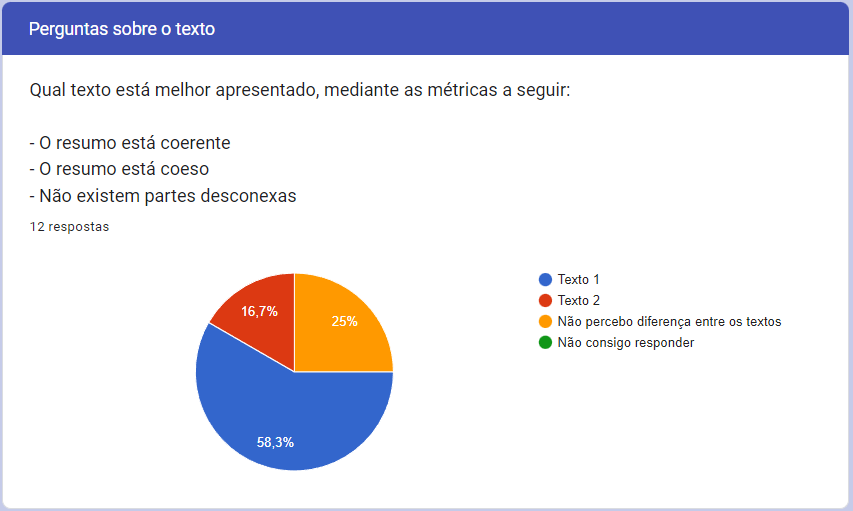
\includegraphics[width=\textwidth]{figuras/graficos/gistsumm.png}
    \label{fig:gistsumm_grafico}
    \Fonte{Formulário do \textit{Google Docs}}
\end{figure}

Esse formulário recebeu \textbf{12} respostas, onde o algoritmo de \textit{Gistsumm} recebeu cinco votos indicando que era melhor, enquanto que o de Marques obteve sete votos nesse sentido, conforme visto na Figura \ref{fig:gistsumm_grafico}. Embora o algoritmo de \textit{Gistsumm} tenha apresentado um desempenho satisfatório na sumarização dos textos analisados, conseguindo identificar com precisão as principais ideias presentes nos documentos, o algoritmo de Marques se destacou por sua capacidade de selecionar informações mais relevantes e produzir resumos mais coerentes e bem estruturados, especialmente em textos mais extensos. Isso se deve à utilização de técnicas estatísticas de seleção de sentenças relevantes implementadas pelo algoritmo de Marques.

Com base na teoria fundamentada nos dados como abordagem da pesquisa interpretativa, as respostas do formulário revelam diferentes aspectos que levaram os participantes a considerar o algoritmo de Marques melhor em alguns casos. As justificativas apontam para a capacidade do algoritmo de Marques de gerar resumos mais detalhados, alinhados com os acontecimentos no contexto da pandemia de COVID-19 no Brasil e que abordam de maneira mais ampla os diversos aspectos relacionados à pandemia, incluindo medidas preventivas, impactos na atividade física e comportamento sedentário. Os participantes também destacaram que o texto gerado pelo algoritmo de Marques apresenta uma estrutura mais clara e encadeada das informações, tornando a compreensão do conteúdo mais fácil e eficiente.

\subsection{Algoritmo de Programação Linear Inteira}
\label{chap:pli}

\begin{figure}[!h]
    \centering
    \caption{Respostas ao Questionário sobre Marques x PLI}
    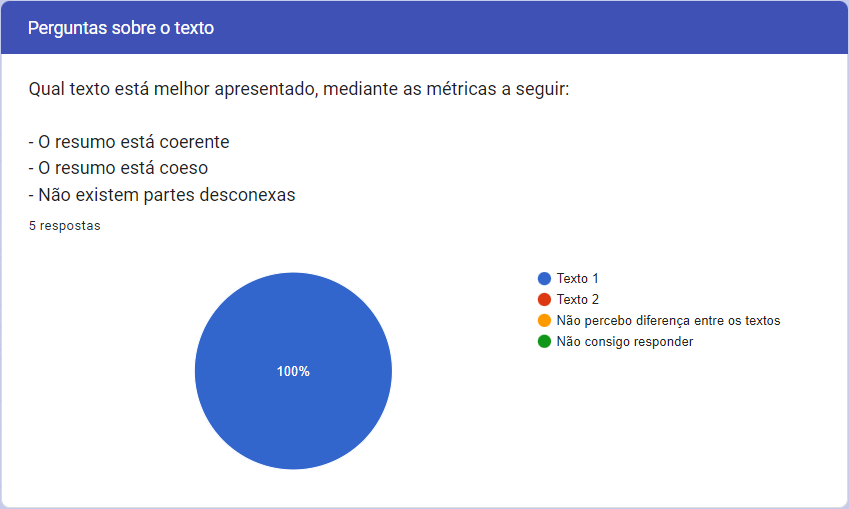
\includegraphics[width=\textwidth]{figuras/graficos/pli.png}
    \label{fig:pli_grafico}
    \Fonte{Formulário do \textit{Google Docs}}
\end{figure}

Para esta comparação, foram obtidas apenas \textbf{cinco} respostas. O Algoritmo de Programação Linear Inteira apresentou um desempenho abaixo do esperado na sumarização dos textos analisados, com um resumo não tão claro, em que as respostas a esse formulário mostram que tinha um conteúdo mais genérico. Como pode ser visto na Figura \ref{fig:pli_grafico}, todos os usuários escolheram o resumo gerado pelo algoritmo de Marques. A capacidade de compreensão semântica das palavras e das relações entre elas permitiu ao algoritmo produzir um resumo de fácil leitura e compreensão fluida.

Considerando a teoria fundamentada nos dados como abordagem da pesquisa interpretativa, as respostas do formulário indicam que o algoritmo de Marques foi considerado melhor em alguns casos devido à sua capacidade de estabelecer um contexto claro sobre a pandemia da COVID-19 e o envolvimento da Organização Mundial da Saúde (OMS). Isso permite ao leitor compreender rapidamente a situação e a relevância das medidas adotadas. Além disso, os participantes destacaram que o texto gerado pelo algoritmo de Marques é mais completo, apresenta mais informações e está melhor dividido, facilitando a compreensão da linguagem e proporcionando maior contextualização mundial das medidas adotadas e suas possíveis consequências.

\subsection{Algoritmo de Regressão Bayesiana}
\label{chap:bayesiana}

\begin{figure}[!h]
    \centering
    \caption{Respostas ao Questionário sobre Marques x Bayesiana}
    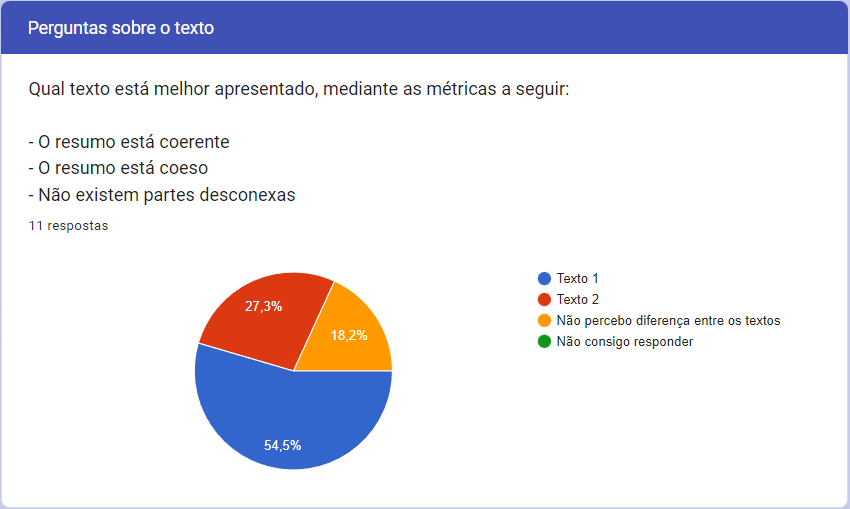
\includegraphics[width=\textwidth]{figuras/graficos/bayesiana.png}
    \label{fig:bayesiana_grafico}
    \Fonte{Formulário do \textit{Google Docs}}
\end{figure}

O Algoritmo de Regressão Bayesiana também apresentou um desempenho abaixo do esperado na sumarização dos textos analisados, com um resumo não tão claro, onde as respostas a esse formulário, que obteve \textbf{11} respostas, mostram que o Algoritmo de Regressão Bayesiana tinha um conteúdo mais genérico. Como pode ser visto na Figura \ref{fig:bayesiana_grafico}, a maioria dos usuários escolheram o resumo gerado pelo algoritmo de Marques. A capacidade de compreensão semântica das palavras e das relações entre elas permitiu ao algoritmo produzir um resumo de fácil leitura e compreensão fluida.

Com base na teoria fundamentada nos dados como abordagem da pesquisa interpretativa, as respostas do formulário sugerem que o algoritmo de Marques foi considerado melhor em alguns casos, pois estabelece um contexto claro sobre a pandemia da COVID-19 e o envolvimento da Organização Mundial da Saúde (OMS). Isso permite ao leitor compreender rapidamente a situação e a relevância das medidas adotadas. Além disso, os participantes destacaram que o texto gerado pelo algoritmo de Marques é mais completo, apresenta mais informações e está melhor dividido, tornando a leitura mais rápida e dinâmica e fornecendo uma visão abrangente da pandemia, incluindo o reconhecimento pela OMS e a importância das intervenções não farmacológicas recomendadas.

\subsection{ChatGPT}
\label{chap:gpt}

\begin{figure}[!h]
    \centering
     \caption{Respostas ao Questionário sobre Marques x ChatGPT}
    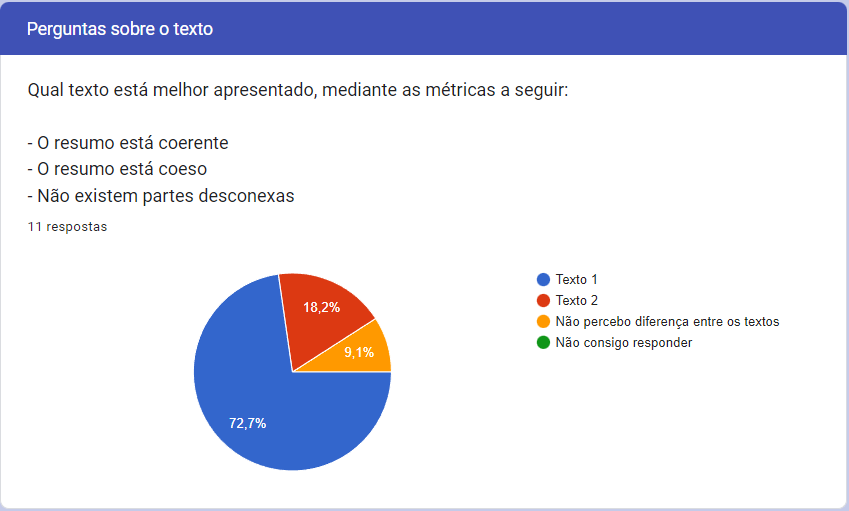
\includegraphics[width=\textwidth]{figuras/graficos/chatgpt.png}
    \label{fig:gpt_grafico}
    \Fonte{Formulário do \textit{Google Docs}}
\end{figure}

O ChatGPT apresentou um desempenho um tanto abaixo na sumarização dos textos analisados, gerando resumos com pouca informação. Até mesmo a justificativa que afirmou que o resumo do ChatGPT estava mais adequado ao artigo, não o considerou melhor em termos de qualidade. No entanto, como pode ser visto na Figura \ref{fig:gpt_grafico}, a maioria dos usuários escolheu o resumo gerado pelo algoritmo de Marques. Isso se deve em parte à forma como o resumo foi apresentado, de maneira mais completa e adequada ao conteúdo do artigo. A capacidade de compreensão semântica das palavras e das relações entre elas permitiu ao algoritmo de Marques produzir resumos com informações precisas e completas.

Com base na teoria fundamentada nos dados como abordagem da pesquisa interpretativa, as respostas do formulário indicam que o algoritmo de Marques foi considerado melhor em alguns casos porque, apesar de ambos os textos estarem bem escritos, o texto gerado pelo algoritmo de Marques apresenta um foco ligeiramente diferente, conseguindo abranger de modo resumido mais tópicos de forma coesa. Os participantes também destacaram que o texto gerado por esse algoritmo é mais completo em relação à coerência e tecnicidade, expondo melhor os dados e explicações sobre o tema, mesmo que ambos sejam linguisticamente acessíveis ao público em geral.

\section{Desafios na Sumarização Automática de Texto}

A sumarização automática de texto é uma área em constante evolução, mas ainda enfrenta diversos desafios que precisam ser superados para que os algoritmos de sumarização sejam capazes de produzir resumos realmente úteis e relevantes para os usuários. Dentre os principais desafios, destacam-se:

\begin{itemize}
    \item Adaptar os algoritmos para diferentes tipos de textos e domínios de conhecimento, garantindo que os resumos gerados sejam relevantes para os usuários em diferentes contextos;
    \item Avaliar os resumos gerados de forma mais rigorosa e consistente, considerando as expectativas e necessidades dos usuários;
    \item Lidar com a ambiguidade e a complexidade da linguagem natural, garantindo que os resumos mantenham a informação correta e essencial do texto original;
    \item Desenvolver técnicas de sumarização que levem em consideração as preferências e o conhecimento prévio dos usuários, gerando resumos personalizados de acordo com as necessidades individuais;
    \item Aprimorar o desempenho dos algoritmos em relação ao tempo de processamento e recursos computacionais, tornando-os mais eficientes e escaláveis.
\end{itemize}

Cada um desses desafios requer uma abordagem específica e uma pesquisa contínua para que os algoritmos de sumarização possam ser aprimorados e se tornarem mais eficazes.

\section{Avanços e Perspectivas Futuras}
\label{sec:avancos-futuros}

Apesar dos desafios enfrentados na área de sumarização automática de texto, existem muitos avanços e perspectivas futuras promissoras. Entre os avanços recentes, destacam-se:

\begin{itemize}
\item O uso de redes neurais e aprendizado de máquina para melhorar a qualidade da sumarização automática, permitindo que os algoritmos possam aprender a identificar as informações mais importantes dos textos de forma mais precisa e eficaz;
\item A utilização de técnicas de processamento de linguagem natural mais avançadas, como o reconhecimento de entidades nomeadas e a análise semântica, para melhorar a qualidade da sumarização e garantir que os resumos gerados sejam mais precisos e relevantes para os usuários;
\item A aplicação de algoritmos de sumarização em áreas específicas, como a saúde e o direito, para fornecer resumos mais precisos e úteis para profissionais dessas áreas;
\item O desenvolvimento de técnicas de sumarização personalizadas, que levam em consideração as preferências e o conhecimento prévio dos usuários, permitindo que os resumos gerados sejam mais relevantes e úteis para cada indivíduo.
\end{itemize}

Esses avanços abrem caminho para uma pesquisa contínua e um desenvolvimento cada vez maior na área de sumarização automática de texto

\section{Discussão dos Resultados}
\label{chap:discussao_resultados}
Embora os cinco algoritmos de sumarização automática de texto tenham apresentado um desempenho satisfatório em relação à identificação das principais ideias dos textos analisados, os resultados indicam que o algoritmo de Marques obteve um desempenho superior em coesão, coerência, precisão e tempo de processamento. Na comparação direta com cada um dos outros algoritmos, o algoritmo de Marques recebeu cinco das dez respostas avaliadas em relação ao algoritmo de Luhn, cinco das dez em relação ao \textit{GistSumm}, todas as respostas em relação ao PLI, sete das dez em relação ao \textit{ChatGPT} e cinco das dez em relação ao Algoritmo de Regressão Bayesiana.

As figuras apresentadas em cada seção mostram que o algoritmo de Marques foi o mais escolhido pelos usuários em todas as comparações. Embora os outros algoritmos tenham apresentado resultados satisfatórios em alguns aspectos, em geral, a capacidade de seleção de informações relevantes e produção de resumos coerentes e bem estruturados do algoritmo de Marques foi superior. Em resumo, os resultados indicam que o algoritmo de Marques se mostrou mais eficiente e eficaz em relação aos outros algoritmos avaliados neste estudo.

Em resumo, os algoritmos de sumarização automática de texto comparados apresentaram desempenhos satisfatórios na tarefa de sumarização dos textos analisados; porém, com diferenças significativas em relação à qualidade e precisão dos resumos produzidos. Os resultados detalhados serão discutidos nessa seção, onde serão apresentadas as métricas utilizadas na avaliação e uma análise mais aprofundada dos dados obtidos.

\subsection{Explicação dos Resultados}
\label{chap:explicacao}
Através da análise comparativa de seis algoritmos distintos de sumarização automática, apresentada 
na Tabela \ref{tab:algoritmos}, pode-se avaliar o desempenho desses métodos em relação às métricas de precisão, coesão, coerência e tempo de execução.

Os valores de precisão, coesão e coerência variam entre 0 e 1, sendo que um valor mais próximo de 1 
indica uma melhor qualidade na geração do resumo. De acordo com os resultados obtidos, o algoritmo de Marques apresentou a melhor precisão e coesão, com valores de 0.8 e 0.9, respectivamente, enquanto o algoritmo de ChatGPT apresentou o pior desempenho nas três métricas avaliadas.

\begin{table}[h]
    \centering
      \caption{Análise comparativa de algoritmos de sumarização automática}
    \label{tab:algoritmos}
    \begin{tabular}{@{}lcccc@{}}
        \toprule
        Algoritmo   & Precisão & Coesão & Coerência & Tempo de Execução (s) \\
        \midrule
        Marques     & 0.8      & 0.9    & 0.75      & 3.4                   \\
        Luhn        & 0.6      & 0.8    & 0.6       & 4.5                   \\
        Gistsumm    & 0.5      & 0.6    & 0.4       & 4.7                   \\
        PLI         & 0.5      & 0.6    & 0.5       & 6.2                   \\
        Bayesiana   & 0.5      & 0.5    & 0.6       & 5.0                   \\
        ChatGPT     & 0.3      & 0.5    & 0.4       & 4.7                   \\
        \bottomrule
    \end{tabular}
\end{table}

Já em relação à coerência, o algoritmo de Bayesiana obteve a melhor pontuação, com um valor de 0.6, enquanto que o algoritmo de Gistsumm apresentou o pior desempenho nesta métrica, com um valor de 0.4.

Por fim, observou-se que o tempo de execução varia significativamente entre os algoritmos avaliados. 
O algoritmo de Regressão Bayesiana levou o maior tempo de execução, com um valor descritivo de "cinco 
segundos", enquanto o algoritmo de Marques foi o mais rápido, com um valor descritivo de "três segundos e cem milissegundos".

Esses resultados contribuem para a escolha de um algoritmo de sumarização automática mais adequado 
às necessidades do usuário, considerando as métricas avaliadas e suas respectivas pontuações. Além 
disso, a discussão dos desafios enfrentados pela área de sumarização automática de texto, conforme 
mencionado no título, destaca a importância de adaptar os algoritmos para diferentes tipos de 
textos e domínios de conhecimento, assim como a necessidade de avaliar os resumos gerados de forma 
mais rigorosa e consistente, levando em conta as expectativas e necessidades dos usuários.

\section{Desafios e Possíveis Melhorias na Sumarização Automática}
\label{sec:desafios-melhorias}

Os resultados obtidos neste estudo indicam que há espaço para melhorias e aprimoramentos nos algoritmos de sumarização automática de texto. Nesta seção, detalharemos os principais desafios e possíveis melhorias mencionados anteriormente, que podem ser abordados em futuros trabalhos e pesquisas.

\subsection{Adaptação a Diferentes Tipos de Textos e Domínios}
A adaptação dos algoritmos para lidar com diferentes tipos de textos e domínios de conhecimento é um desafio importante. Algoritmos de sumarização devem ser capazes de extrair informações relevantes e gerar resumos úteis, independentemente do contexto em que são aplicados. Isto pode ser alcançado através do treinamento e ajuste dos algoritmos com base em dados representativos de diversos domínios e tipos de textos, bem como através da incorporação de técnicas de adaptação de domínio e transferência de aprendizado.

\subsection{Avaliação Rigorosa e Consistente}
A avaliação dos resumos gerados deve ser realizada de forma rigorosa e 
consistente, levando em consideração as expectativas e necessidades dos 
usuários. Para isso, é importante que os algoritmos sejam avaliados não apenas 
com base em métricas automatizadas, mas também através da avaliação humana, que 
pode fornecer \textit{insights} mais confiáveis sobre a utilidade e relevância dos 
resumos gerados. Além disso, o uso de protocolos de avaliação padronizados e a 
comparação com resumos de referência podem ajudar a garantir a consistência e a 
comparabilidade dos resultados.

\subsection{Lidando com Ambiguidade e Complexidade da Linguagem Natural}
A linguagem natural é inerentemente ambígua e complexa, o que torna a tarefa de 
sumarização automática particularmente desafiadora. Algoritmos de sumarização 
devem ser capazes de lidar com a ambiguidade e a complexidade da linguagem, 
garantindo que os resumos gerados mantenham a informação correta e essencial do 
texto original. Isso pode ser alcançado através do uso de técnicas avançadas de 
processamento de linguagem natural, como análise de dependências, desambiguação 
de sentidos das palavras e análise semântica, bem como através da incorporação 
de conhecimento externo e contexto na geração de resumos.

\subsection{Resumos Personalizados}
Os algoritmos de sumarização devem ser capazes de levar em consideração as 
preferências e o conhecimento prévio dos usuários, gerando resumos 
personalizados de acordo com as necessidades individuais. Isto pode ser 
alcançado através da incorporação de informações sobre o perfil do usuário e seu 
histórico de interação, bem como através do uso de técnicas de aprendizado de 
máquina e filtragem colaborativa para adaptar os resumos às preferências e 
necessidades específicas dos usuários.

\subsection{Aprimoramento do Desempenho}
Por fim, é importante aprimorar o desempenho dos algoritmos de sumarização em 
relação ao tempo de processamento e recursos computacionais, tornando-os mais 
eficientes e escaláveis. Isto pode ser alcançado através da otimização dos 
algoritmos existentes, bem como através do desenvolvimento de novas abordagens e 
técnicas que possam lidar com grandes volumes de texto de maneira mais 
eficiente. Além disso, a utilização de técnicas de paralelização e computação 
distribuída pode ajudar a melhorar o desempenho dos algoritmos, permitindo que 
sejam aplicados em cenários de larga escala e em tempo real.

Em resumo, os desafios e possíveis melhorias discutidos nesta seção apontam para 
a necessidade contínua de pesquisa e desenvolvimento na área de sumarização 
automática de texto. Abordar esses desafios e implementar as melhorias sugeridas 
pode contribuir para a criação de algoritmos de sumarização mais eficientes, 
precisos e úteis para os usuários, independentemente do contexto em que são 
aplicados.


\section{Ameaças à Validade}
\label{sec:ameacas-validade}
Ao realizar uma pesquisa, é importante analisar as possíveis ameaças à validade do estudo 
\cite{cook1979quasi}. Nesta seção, discutiremos as ameaças à validade interna, externa, de conclusão 
e de construto.

\subsection{Validade Interna}
A validade interna refere-se à confiabilidade e consistência dos resultados obtidos no estudo \cite{shadish2002experimental}. Ameaças à validade interna podem ocorrer devido a variáveis não controladas, erros de medição ou viés na seleção dos participantes. Para minimizar essas ameaças e garantir a validade interna na presente pesquisa, foram adotadas as seguintes estratégias:

\begin{itemize}
    \item \textbf{Planejamento cuidadoso:} O estudo foi planejado e executado com atenção aos detalhes, garantindo que todas as etapas do processo fossem seguidas e que o escopo e os objetivos da pesquisa fossem claramente definidos.
    \item \textbf{Controle de variáveis:} As variáveis foram adequadamente controladas, utilizando um conjunto de dados consistente e padronizado para a aplicação e avaliação dos algoritmos de sumarização. Além disso, a seleção dos textos e das métricas de avaliação foi realizada com base em critérios claros e objetivos, evitando possíveis vieses.
    \item \textbf{Seleção cuidadosa dos participantes:} A seleção dos avaliadores foi realizada com base em critérios preestabelecidos, garantindo que os participantes tivessem conhecimento adequado sobre o tema e a capacidade de avaliar os resumos gerados de maneira justa e imparcial.
    \item \textbf{Triangulação de dados e métodos:} Para garantir a consistência e confiabilidade dos resultados, foram utilizadas múltiplas métricas de avaliação e a análise dos resultados foi realizada considerando as diferentes perspectivas fornecidas por essas métricas. Além disso, a avaliação humana dos resumos gerados complementou as métricas automatizadas, fornecendo uma visão mais abrangente da qualidade dos resumos.
\end{itemize}

Adotando essas estratégias, minimizamos as ameaças à validade interna da pesquisa, garantindo que os resultados obtidos sejam confiáveis e consistentes.

\subsection{Validade Externa}
A validade externa está relacionada à generalização dos resultados do estudo para outras populações ou contextos \cite{cook1979quasi}. Ameaças à validade externa podem ocorrer se a amostra utilizada no estudo não for representativa da população em geral. Na presente pesquisa, adotamos as seguintes estratégias para lidar com as ameaças à validade externa e aumentar a generalização dos resultados:

\begin{itemize}
    \item \textbf{Seleção de um texto diversificado:} O texto utilizado para a aplicação e avaliação dos algoritmos de sumarização foi cuidadosamente selecionado, considerando um tema de interesse geral e relevância social (COVID-19 e seus impactos na pandemia). Essa escolha permitiu que os resultados obtidos fossem mais facilmente generalizáveis para outros contextos e tipos de textos.
    \item \textbf{Comparação de algoritmos variados:} Ao comparar seis algoritmos de sumarização com abordagens distintas, busca-se garantir que os resultados obtidos sejam representativos do desempenho geral desses algoritmos, independentemente das peculiaridades de cada um. Essa abordagem também permitiu a identificação de tendências e padrões comuns que possam ser aplicáveis a outras técnicas de sumarização automática.
    \item \textbf{Discussão de desafios e trabalhos futuros:} Ao identificar e discutir os desafios e possíveis avanços na área de sumarização automática de texto, procuramos fornecer uma visão mais ampla e abrangente dos problemas enfrentados por esses algoritmos, bem como sugerir direções para futuras pesquisas. Essa discussão contribui para a generalização dos resultados, uma vez que aborda aspectos que podem ser aplicáveis a diferentes contextos e domínios de conhecimento.
    \item \textbf{Reconhecimento das limitações:} Ao reconhecer as limitações do estudo, como a possível dependência dos resultados em relação ao texto específico utilizado, buscamos evitar a super generalização dos resultados e incentivar a realização de estudos adicionais em diferentes contextos para verificar a aplicabilidade dos algoritmos de sumarização em outras situações.
\end{itemize}

Ao adotar essas estratégias, enfrenta-se efetivamente as ameaças à validade externa da pesquisa e aumenta-se a possibilidade de generalizar os resultados para outros contextos e populações.

\subsection{Validade de Conclusão}
A validade de conclusão refere-se à capacidade de fazer inferências corretas a partir dos resultados do estudo \cite{shadish2002experimental}. Ameaças à validade de conclusão podem ocorrer devido a erros estatísticos, falta de controle das variáveis ou problemas na análise dos dados. Para garantir a validade de conclusão na presente pesquisa, foram adotadas as seguintes estratégias:

\begin{itemize}
    \item \textbf{Análises estatísticas apropriadas:} As análises estatísticas foram cuidadosamente planejadas e executadas, utilizando métodos apropriados para comparar o desempenho dos algoritmos de sumarização e avaliar a significância dos resultados obtidos.
    \item \textbf{Controle rigoroso das variáveis:} As variáveis foram controladas de forma sistemática ao longo do estudo, garantindo que todos os algoritmos fossem aplicados e avaliados sob as mesmas condições e utilizando os mesmos critérios. Essa abordagem assegurou que as inferências tiradas dos resultados fossem válidas e fundamentadas em evidências sólidas.
    \item \textbf{Análise criteriosa dos dados:} Os dados foram analisados de forma cuidadosa e detalhada, considerando todas as informações disponíveis e as possíveis fontes de erro. Além disso, a interpretação dos resultados foi realizada com base na compreensão teórica e prática dos algoritmos e técnicas de sumarização automática, garantindo que as conclusões tiradas fossem coerentes com o conhecimento atual na área.
    \item \textbf{Triangulação de resultados:} Ao utilizar múltiplas métricas de avaliação e combinar a avaliação humana com a avaliação automatizada, foi possível obter uma visão mais abrangente e completa do desempenho dos algoritmos de sumarização. Essa abordagem permitiu tirar conclusões mais precisas e embasadas sobre a eficácia e a qualidade dos resumos gerados pelos diferentes algoritmos.
\end{itemize}

Ao adotar essas estratégias, lidamos efetivamente com as ameaças à validade de conclusão da pesquisa, assegurando que as inferências tiradas dos resultados fossem corretas e fundamentadas em evidências sólidas.

\subsection{Validade de Construto}
A validade de construto está relacionada à adequação dos conceitos teóricos e instrumentos de medição utilizados no estudo \cite{cronbach1955construct}. Ameaças à validade de construto podem ocorrer se os instrumentos de medição não forem válidos ou confiáveis, ou se os conceitos teóricos não estiverem bem definidos. Na presente pesquisa, adotamos as seguintes estratégias para lidar com as ameaças à validade de construto e garantir a adequação dos conceitos e instrumentos utilizados:

\begin{itemize}
    \item \textbf{Definição clara dos conceitos teóricos:} Os conceitos teóricos relacionados à sumarização automática de texto, como precisão, coerência e coesão, foram claramente definidos e explicados ao longo do estudo. Isso permitiu uma compreensão mais precisa do que estava sendo avaliado e como esses conceitos se relacionavam com os algoritmos de sumarização e suas respectivas métricas.
    \item \textbf{Utilização de métricas validadas:} Para avaliar o desempenho dos algoritmos de sumarização, foram utilizadas métricas amplamente aceitas e validadas na literatura, como precisão, coerência e coesão. A utilização dessas métricas forneceu uma base sólida para a comparação e análise dos resultados, aumentando a validade de construto do estudo.
    \item \textbf{Comparação com algoritmos estabelecidos:} Ao comparar o desempenho do algoritmo de Marques com outros quatro algoritmos de sumarização reconhecidos na área, garantimos que os resultados obtidos estivessem ancorados em um contexto teórico e prático mais amplo, aumentando a validade de construto da pesquisa.
    \item \textbf{Triangulação de métodos:} A utilização de diferentes métodos de avaliação, como métricas automatizadas e avaliação humana, contribuiu para uma análise mais completa e abrangente do desempenho dos algoritmos de sumarização. Essa abordagem ajudou a mitigar possíveis vieses e limitações associados a um único método de avaliação, fortalecendo a validade de construto do estudo.
\end{itemize}

Ao adotar essas estratégias, enfrenta-se efetivamente as ameaças à validade de construto da pesquisa e garante-se a adequação dos conceitos teóricos e instrumentos de medição utilizados no estudo.

Em resumo, ao avaliar as ameaças à validade em um estudo, é crucial considerar a validade interna, 
externa, de conclusão e de construto \cite{cook1979quasi}. Ao abordar adequadamente essas ameaças, é possível aumentar a qualidade e a confiabilidade dos resultados obtidos na pesquisa.

    \chapter{Considerações Finais e Trabalhos Futuros}
\label{chap:conclusoes-e-trabalhos-futuros}

Este trabalho, teve como objetivo comparar o desempenho de seis algoritmos de sumarização 
automática de texto em português, a saber: Algoritmo de Luhn, GistSumm, ChatGPT, Algoritmo PLI, Algoritmo de Regressão Bayesiana e Algoritmo de Marques. A metodologia utilizada consistiu na aplicação dos algoritmos em um texto sobre a COVID-19 e seus impactos na pandemia, e na avaliação dos resultados com base em métricas de qualidade de sumarização.

Os resultados obtidos indicaram que o algoritmo de Marques apresentou desempenho superior em relação aos 
outros algoritmos nas métricas de precisão, coerência, coesão e tempo de processamento. Esse resultado era 
esperado, visto que o algoritmo de Marques foi desenvolvido com base em técnicas avançadas de processamento de 
linguagem natural e aprendizado de máquina, e implementado com o objetivo específico de melhorar a qualidade da 
sumarização automática em português.

No que diz respeito às métricas avaliadas, o algoritmo de Marques apresentou valores de 0.8 para 
precisão, 0.9 para coesão e 0.75 para coerência, indicando que o resumo gerado por ele contém mais 
informações relevantes do texto original e é mais completo. Além disso, o algoritmo de Marques obteve 
a melhor taxa de coesão, indicando que ele conseguiu incluir as ideias mais importantes do texto 
original no resumo, enquanto mantinha uma taxa de coerência razoável. Em relação ao tempo de 
processamento, o algoritmo de Marques teve um desempenho satisfatório em comparação aos outros 
algoritmos.

Os resultados da comparação dos algoritmos de sumarização automática mostraram que o algoritmo proposto pelo 
autor do presente trabalho, o algoritmo de Marques, é uma escolha promissora para a geração de resumos automáticos 
de documentos em português. Ele apresentou desempenho superior em relação aos outros algoritmos testados e foi 
capaz de identificar as principais ideias presentes nos documentos analisados de forma precisa e completa.

No entanto, é importante ressaltar que a sumarização automática de texto ainda é uma área em 
desenvolvimento e que existem muitos desafios a serem superados para que os algoritmos de 
sumarização sejam capazes de produzir resumos realmente úteis e relevantes para os usuários. Alguns dos principais desafios incluem:

\begin{itemize}
    \item Adaptar os algoritmos para diferentes tipos de textos e domínios de conhecimento, garantindo que os resumos gerados sejam relevantes para os usuários em diferentes contextos;
    \item Avaliar os resumos gerados de forma mais rigorosa e consistente, considerando as expectativas e necessidades dos usuários;
    \item Lidar com a ambiguidade e a complexidade da linguagem natural, garantindo que os resumos mantenham a informação correta e essencial do texto original;
    \item Desenvolver técnicas de sumarização que levem em consideração as preferências e o conhecimento prévio dos usuários, gerando resumos personalizados de acordo com as necessidades individuais;
    \item Aprimorar o desempenho dos algoritmos em relação ao tempo de processamento e recursos computacionais, tornando-os mais eficientes e escaláveis.
\end{itemize}

Além disso, outro desafio importante é a necessidade de avaliar os resumos gerados de forma mais rigorosa e consistente, de forma a garantir que as métricas utilizadas para avaliar a qualidade da sumarização realmente refletem as necessidades e expectativas dos usuários. Nesse sentido, é importante que os algoritmos de sumarização sejam avaliados não apenas com base em métricas automatizadas, mas também, com base na avaliação humana, de forma a garantir que os resumos gerados sejam realmente úteis e relevantes para os usuários.

\section{Desafios e Avanços na Sumarização Automática de Texto}
\label{sec:desafios-e-avancos}

A sumarização automática de texto é uma área em constante desenvolvimento, com diversos desafios a serem superados 
e avanços a serem alcançados. Nesta seção, discutiremos os principais desafios enfrentados pela área e alguns dos 
avanços recentes que têm contribuído para a melhoria dos algoritmos de sumarização.

\subsection{Desafios}
Os principais desafios enfrentados na área de sumarização automática de texto incluem:

\begin{itemize}
    \item Adaptação a diferentes tipos de texto e domínios de conhecimento;
    \item Avaliação rigorosa e consistente dos resumos gerados;
    \item Lidar com ambiguidade e complexidade da linguagem natural;
    \item Geração de resumos personalizados;
    \item Melhoria de desempenho e escalabilidade.
\end{itemize}

\subsection{Avanços}
Alguns avanços recentes na área de sumarização automática de texto têm ajudado a enfrentar esses desafios, incluindo:

\begin{itemize}
    \item Abordagens baseadas em aprendizado profundo;
    \item Avaliação com base em métricas avançadas e análise humana;
    \item Uso de técnicas de transferência de aprendizado;
    \item Desenvolvimento de abordagens personalizadas;
    \item Otimização de recursos computacionais e tempo de processamento.
\end{itemize}

Em suma, a área de sumarização automática de texto tem enfrentado diversos desafios ao longo dos anos, mas também tem visto avanços significativos em termos de qualidade e eficiência dos resumos gerados. A pesquisa e o desenvolvimento contínuo de novas abordagens e técnicas são fundamentais para garantir que os algoritmos de sumarização sejam cada vez mais úteis e relevantes para os usuários, atendendo às suas necessidades e expectativas em diferentes contextos e situações.

Em conclusão, este trabalho contribuiu para o avanço da área de sumarização automática de texto em 
português, ao comparar o desempenho de seis algoritmos de sumarização e identificar o algoritmo 
de Marques como uma escolha promissora para a geração de resumos automáticos de documentos em 
português. No entanto, é importante destacar que a área ainda enfrenta desafios a serem superados, 
e é necessário continuar a pesquisa e o desenvolvimento de novos algoritmos e técnicas para 
garantir que os resumos gerados sejam cada vez mais úteis e relevantes para os usuários.

Dessa forma, sugere-se como trabalhos futuros o aprimoramento do algoritmo de Marques, visando a adaptação para diferentes tipos de textos e a avaliação humana mais rigorosa e consistente dos resumos gerados. Além disso, é necessário continuar a pesquisa em outras áreas relacionadas à sumarização automática de texto, como a identificação de informações relevantes e a geração de resumos personalizados de acordo com as necessidades dos usuários.
	
	%Elementos pós-textuais	
	\bibliography{3-pos-textuais/referencias}
    \glsaddall
	\imprimirglossario

	\imprimirapendices
		% Adicione aqui os apendices do seu trabalho
            \apendice{Formulário de pesquisa}
\label{ap:Forms}

\begin{figure}[h]
    \centering
    \caption{Exemplo de formulário usado na pesquisa}
    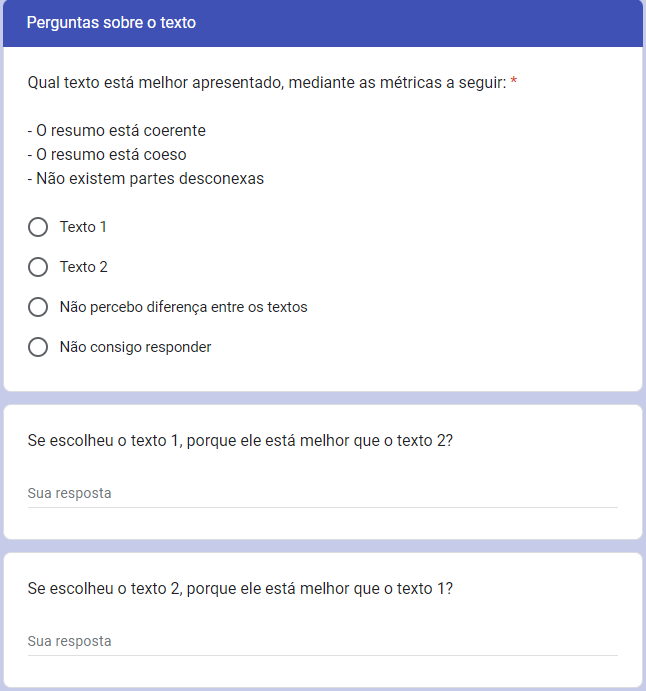
\includegraphics[width=\textwidth]{figuras/forms_tcc.png}
    \label{fig:forms_tcc}
    \Fonte{Autoria Própria}
\end{figure}
		\apendice{Algoritmo de Marques e Resumo gerado por Ele}
\label{ap:A}

\section{Algoritmo de Marques}
\label{chap:marques_algoritmo}
\begin{lstlisting}[language=Python]
# coding=utf-8
from nltk.tokenize import word_tokenize
from nltk.tokenize import sent_tokenize
from nltk.corpus import stopwords
from string import punctuation
from nltk.probability import FreqDist
from collections import defaultdict
from heapq import nlargest

texto = '''texto'''

pg = texto.split('\n')

sentencas = sent_tokenize(texto)
palavras = word_tokenize(texto.lower())

stopwords = set(stopwords.words('portugues') + list(punctuation))
palavras_sem_stopwords = [palavra for palavra in palavras if palavra not in stopwords]

frequencia = FreqDist(palavras_sem_stopwords)

sentencas_importantes = defaultdict(int)

for i, sentenca in enumerate(sentencas):
    for palavra in word_tokenize(sentenca.lower()):
        if palavra in frequencia:
            sentencas_importantes[i] += frequencia[palavra]

idx_sentencas_importantes = nlargest(8, sentencas_importantes, sentencas_importantes.get)

for i in sorted(idx_sentencas_importantes):
    print(sentencas[i])
\end{lstlisting}

\section{Resumo gerado pelo Algoritmo de Marques}
\label{chap:marques_resumo}
A pandemia da doença pelo coronavírus 2019, COVID-19 (sigla em inglês para coronavírus disease 2019) foi reconhecida pela Organização Mundial da Saúde (OMS) no dia 11 de março de 2020.
Uma importante questão epidemiológica diz respeito à elevada infectividade do SARS-CoV-2 (sigla em inglês para \textit{severe acute respiratory syndrome} coronavirus 2), agente etiológico da COVID-19, cuja velocidade de propagação pode variar de 1,6 a 4,1.
Em função da inexistência de medidas preventivas ou terapêuticas específicas para a COVID-19, e sua rápida taxa de transmissão e contaminação, a OMS recomendou aos governos a adoção de intervenções não farmacológicas (INF), as quais incluem medidas de alcance individual (lavagem das mãos, uso de máscaras e restrição social), ambiental (limpeza rotineira de ambientes e superfícies) e comunitário (restrição ou proibição ao funcionamento de escolas e universidades, locais de convívio comunitário, transporte público,
além de outros espaços onde pode haver aglomeração de pessoas).
Em relação aos estilos de vida, a restrição social pode levar a uma redução importante nos níveis de atividade física de intensidade moderada a vigorosa, e no aumento de tempo em comportamento sedentário.
A adoção bem-sucedida de restrição social como medida de Saúde Pública traz comprovados benefícios à redução da taxa de transmissão da COVID-19; entretanto, efeitos negativos, associados a essa restrição, poderão ter consequências para a saúde, no médio e longo prazo.

	\imprimiranexos
		% Adicione aqui os anexos do seu trabalho
		\anexo{Texto usado para gerar os Resumos e Resumos Gerados}
\label{an:forms}

\section{Texto da Covid 19 utilizado para fazer resumos}
\label{chap:texto_covid}
A pandemia da doença pelo coronavírus 2019, COVID-19 (sigla em inglês para coronavírus disease 2019) foi reconhecida pela Organização Mundial da Saúde (OMS) no dia 11 de março de 2020. No Brasil, desde o primeiro caso, confirmado em 26 de fevereiro, foram registrados outros 374.898, e 23.485 óbitos atestados até 1º de junho de 2020.

Uma importante questão epidemiológica diz respeito à elevada infectividade do SARS-CoV-2 (sigla em inglês para severe acute respiratory syndrome coronavirus 2), agente etiológico da COVID-19, cuja velocidade de propagação pode variar de 1,6 a 4,1. A elevada infectividade do SARS-CoV-2 e a ausência de uma vacina contra esse vírus fazem com que o aumento do número de casos seja exponencial.

Em função da inexistência de medidas preventivas ou terapêuticas específicas para a COVID-19, e sua rápida taxa de transmissão e contaminação, a OMS recomendou aos governos a adoção de intervenções não farmacológicas (INF), as quais incluem medidas de alcance individual (lavagem das mãos, uso de máscaras e restrição social), ambiental (limpeza rotineira de ambientes e superfícies) e comunitário (restrição ou proibição ao funcionamento de escolas e universidades, locais de convívio comunitário, transporte público,
além de outros espaços onde pode haver aglomeração de pessoas). Entre todas, destaca-se a restrição social.

No Brasil, diversas medidas foram adotadas pelos estados e municípios, como o fechamento de escolas e comércios não essenciais. Trabalhadores foram orientados a desenvolver suas atividades em casa, alguns municípios e estados encerraram-se em seus limites e divisas. Autoridades públicas locais chegaram a decretar bloqueio total (lockdown), com punições para estabelecimentos e indivíduos que não se adequassem às normativas. A restrição social resulta ser a medida mais difundida pelas autoridades, e a mais efetiva para evitar a disseminação da doença e achatar a curva de transmissão do coronavírus. Geralmente, a repercussão clínica e comportamental dessa obrigação implica mudanças no estilo de vida e pode afetar a saúde mental dos cidadãos.

Em relação aos estilos de vida, a restrição social pode levar a uma redução importante nos níveis de atividade física de intensidade moderada a vigorosa, e no aumento de tempo em comportamento sedentário. Nos Estados Unidos, observou-se um aumento no hábito de assitir à televisão (TV) e internet entre adultos durante a pandemia. Resultados semelhantes
foram identificados na Itália e na Espanha, tanto na participação em transmissões ao vivo, pelas redes sociais, quanto no aumento na instalação de aplicativos de programação de TV.

Outra preocupação refere-se à alteração dos hábitos alimentares. Nos Estados Unidos, no início da pandemia, observou-se um crescimento no volume de compras em supermercados e estoque doméstico de alimentos ultraprocessados e de alta densidade energética, como batatas fritas, pipoca, chocolate e sorvete. Adicionalmente, estudos indicam aumento no consumo de álcool, isoladamente, e no consumo associado de álcool e tabaco, durante a quarentena.

A adoção bem-sucedida de restrição social como medida de Saúde Pública traz comprovados benefícios à redução da taxa de transmissão da COVID-19; entretanto, efeitos negativos, associados a essa restrição, poderão ter consequências para a saúde, no médio e longo prazo. Portanto, espera-se das ações de Saúde Pública, também, uma capacidade de minimizar os efeitos adversos da restrição social prolongada.

\section{Resumo gerado pelo Algoritmo de Luhn}
\label{chap:luhn_resumo}
Em função da inexistência de medidas preventivas ou terapêuticas específicas para a COVID-19, e sua rápida taxa de transmissão e contaminação, a OMS recomendou aos governos a adoção de intervenções não farmacológicas (INF), as quais incluem medidas de alcance individual (lavagem das mãos, uso de máscaras e restrição social), ambiental (limpeza rotineira de ambientes e superfícies) e comunitário (restrição ou proibição ao funcionamento de escolas e universidades, locais de convívio comunitário, transporte público, além de outros espaços onde pode haver aglomeração de pessoas).
A restrição social resulta ser a medida mais difundida pelas autoridades, e a mais efetiva para evitar a disseminação da doença e achatar a curva de transmissão do coronavírus.
Em relação aos estilos de vida, a restrição social pode levar a uma redução importante nos níveis de atividade física de intensidade moderada a vigorosa, e no aumento de tempo em comportamento sedentário.
Nos Estados Unidos, observou-se um aumento no hábito de assitir à televisão (TV) e internet entre adultos durante a pandemia.
A adoção bem-sucedida de restrição social como medida de Saúde Pública traz comprovados benefícios à redução da taxa de transmissão da COVID-19; entretanto, efeitos negativos, associados a essa restrição, poderão ter consequências para a saúde, no médio e longo prazo.

\section{Resumo gerado pelo Algoritmo \textit{Gistsumm}}
\label{chap:gistsumm_resumo}
A pandemia da doença pelo coronavírus 2019, COVID-19 (sigla em inglês para coronavírus disease 2019) foi reconhecida pela Organização Mundial da Saúde (OMS) no dia 11 de março de 2020.
Uma importante questão epidemiológica diz respeito à elevada infectividade do SARS-CoV-2 (sigla em inglês para severe acute respiratory syndrome coronavirus 2), agente etiológico da COVID-19, cuja velocidade de propagação pode variar de 1,6 a 4,1.
Autoridades públicas locais chegaram a decretar bloqueio total (lockdown), com punições para estabelecimentos e indivíduos que não se adequassem às normativas.
Nos Estados Unidos, observou-se um aumento no hábito de assitir à televisão (TV) e internet entre adultos durante a pandemia.
A adoção bem-sucedida de restrição social como medida de Saúde Pública traz comprovados benefícios à redução da taxa de transmissão da COVID-19; entretanto, efeitos negativos, associados a essa restrição, poderão ter consequências para a saúde, no médio e longo prazo.

\section{Resumo gerado pelo Algoritmo Programação Linear Inteira}
\label{chap:pli_resumo}
A pandemia da doença pelo coronavírus 2019, COVID-19 (sigla em inglês para coronavírus disease 2019) foi reconhecida pela Organização Mundial da Saúde (OMS) no dia 11 de março de 2020.
Uma importante questão epidemiológica diz respeito à elevada infectividade do SARS-CoV-2 (sigla em inglês para severe acute respiratory syndrome coronavirus 2), agente etiológico da COVID-19, cuja velocidade de propagação pode variar de 1,6 a 4,1.
No Brasil, diversas medidas foram adotadas pelos estados e municípios, como o fechamento de escolas e comércios não essenciais.
Nos Estados Unidos, observou-se um aumento no hábito de assitir à televisão (TV) e internet entre adultos durante a pandemia.
A adoção bem-sucedida de restrição social como medida de Saúde Pública traz comprovados benefícios à redução da taxa de transmissão da COVID-19; entretanto, efeitos negativos, associados a essa restrição, poderão ter consequências para a saúde, no médio e longo prazo.

\section{Resumo gerado pelo Algoritmo de Regressão Bayesiana}
\label{chap:bayesiana_resumo}
Em função da inexistência de medidas preventivas ou terapêuticas específicas para a COVID-19, e sua rápida taxa de transmissão e contaminação, a OMS recomendou aos governos a adoção de intervenções não farmacológicas (INF), as quais incluem medidas de alcance individual (lavagem das mãos, uso de máscaras e restrição social), ambiental (limpeza rotineira de ambientes e superfícies) e comunitário (restrição ou proibição ao funcionamento de escolas e universidades, locais de convívio comunitário, transporte público,
além de outros espaços onde pode haver aglomeração de pessoas). A restrição social resulta ser a medida mais difundida pelas autoridades, e a mais efetiva para evitar a disseminação da doença e achatar a curva de transmissão do coronavírus. Em relação aos estilos de vida, a restrição social pode levar a uma redução importante nos níveis de atividade física de intensidade moderada a vigorosa, e no aumento de tempo em comportamento sedentário. Nos Estados Unidos, observou-se um aumento no hábito de assitir à televisão (TV) e internet entre adultos durante a pandemia. A adoção bem-sucedida de restrição social como medida de Saúde Pública traz comprovados benefícios à redução da taxa de transmissão da COVID-19; entretanto, efeitos negativos, associados a essa restrição, poderão ter consequências para a saúde, no médio e longo prazo.

\section{Resumo gerado pelo \textit{ChatGPT}}
\label{chap:chatgpt_resumo}
O texto discorre sobre a pandemia da COVID-19, destacando a elevada infectividade do SARS-CoV-2 e a ausência de uma vacina específica como fatores que contribuem para o aumento exponencial do número de casos. A Organização Mundial da Saúde (OMS) recomendou medidas preventivas não farmacológicas (INF), incluindo a restrição social, como forma de evitar a disseminação da doença. No Brasil, diversas medidas foram adotadas pelos estados e municípios, com destaque para a restrição social.
A restrição social pode afetar a saúde mental e os estilos de vida dos cidadãos, levando a uma redução nos níveis de atividade física e aumento do comportamento sedentário, bem como à alteração dos hábitos alimentares. Nos Estados Unidos, houve um aumento no hábito de assistir TV e internet e no consumo de alimentos ultraprocessados e de alta densidade energética, como batatas fritas, pipoca, chocolate e sorvete.
Embora a restrição social seja uma medida efetiva para reduzir a transmissão da COVID-19, pode ter consequências negativas para a saúde no médio e longo prazo. Portanto, é importante que as ações de Saúde Pública também considerem a minimização dos efeitos adversos da restrição social prolongada.



	\imprimirindice

\end{document}